\documentclass[a4paper, 11pt, oneside, landscape]{article}
\usepackage[T1]{fontenc}
\usepackage{ebgaramond}
% Load encoding definitions (after font package)
\usepackage{textalpha}
\usepackage[dvipsnames]{xcolor}
\usepackage{eso-pic,graphicx}
\usepackage[top=33mm, bottom=37mm, outer=27mm, inner=27mm]{geometry}
\setlength{\columnsep}{90pt}

% Babel package:
\usepackage[main=french,polutonikogreek]{babel}
\babelprovide[import]{hebrew}
\usepackage{arabtex}
\usepackage{cjhebrew}
\usepackage{svg}
\usepackage{listings}
\lstset{basicstyle=\ttfamily}
\usepackage{bbding}
% With XeTeX$\$LuaTeX, load fontspec after babel to use Unicode
% fonts for Latin script and LGR for Greek:
\ifdefined\luatexversion \usepackage{fontspec}\fi
\ifdefined\XeTeXrevision \usepackage{fontspec}\fi

% "Lipsiakos" italic font `cbleipzig`:
\newcommand*{\lishape}{\fontencoding{LGR}\fontfamily{cmr}%
		       \fontshape{li}\selectfont}
\DeclareTextFontCommand{\textli}{\lishape}

\usepackage{booktabs}
\usepackage{graphicx}
\setlength{\emergencystretch}{15pt}
\graphicspath{ {./ } }
\usepackage[figurename=]{caption}
\usepackage{float}
\usepackage{fancyhdr}
\usepackage{microtype}
\usepackage{setspace}
\onehalfspacing

\makeatletter % change only the display of \thepage, but not \thepage itself:
\patchcmd{\ps@plain}{\thepage}{\bfseries\color{White}{\thepage}}{}{}
\makeatother

\color{White}
%define custom symbols
\newcommand*\svgAAAA{\includesvg[height=1em]{white/svg001.svg}}
\newcommand*\svgAAAB{\includesvg[height=1em]{white/svg002.svg}}
\newcommand*\svgAAAC{\includesvg[height=1em]{white/svg003.svg}}
\newcommand*\svgAAAD{\includesvg[height=1em]{white/svg004.svg}}
\newcommand*\svgAAAE{\includesvg[height=1em]{white/svg005.svg}}
\newcommand*\svgAAAF{\includesvg[height=1em]{white/svg006.svg}}
\newcommand*\svgAAAG{\includesvg[height=0.5em]{white/svg007.svg}}
\newcommand*\svgAAAH{\includesvg[height=1em]{white/svg008.svg}}
\newcommand*\svgAAAI{\includesvg[height=1em]{white/svg009.svg}}
\newcommand*\svgAAAJ{\includesvg[height=1em]{white/svg010.svg}}
\newcommand*\svgAAAK{\raisebox{-0.8ex}{\includesvg[height=1em]{white/svg011.svg}}}
\newcommand*\svgAAAL{\includesvg[height=1em]{white/svg012.svg}}
\newcommand*\svgAAAM{\raisebox{-0.8ex}{\includesvg[height=1em]{white/svg013.svg}}}

\begin{document}

\bfseries
\AddToShipoutPictureBG{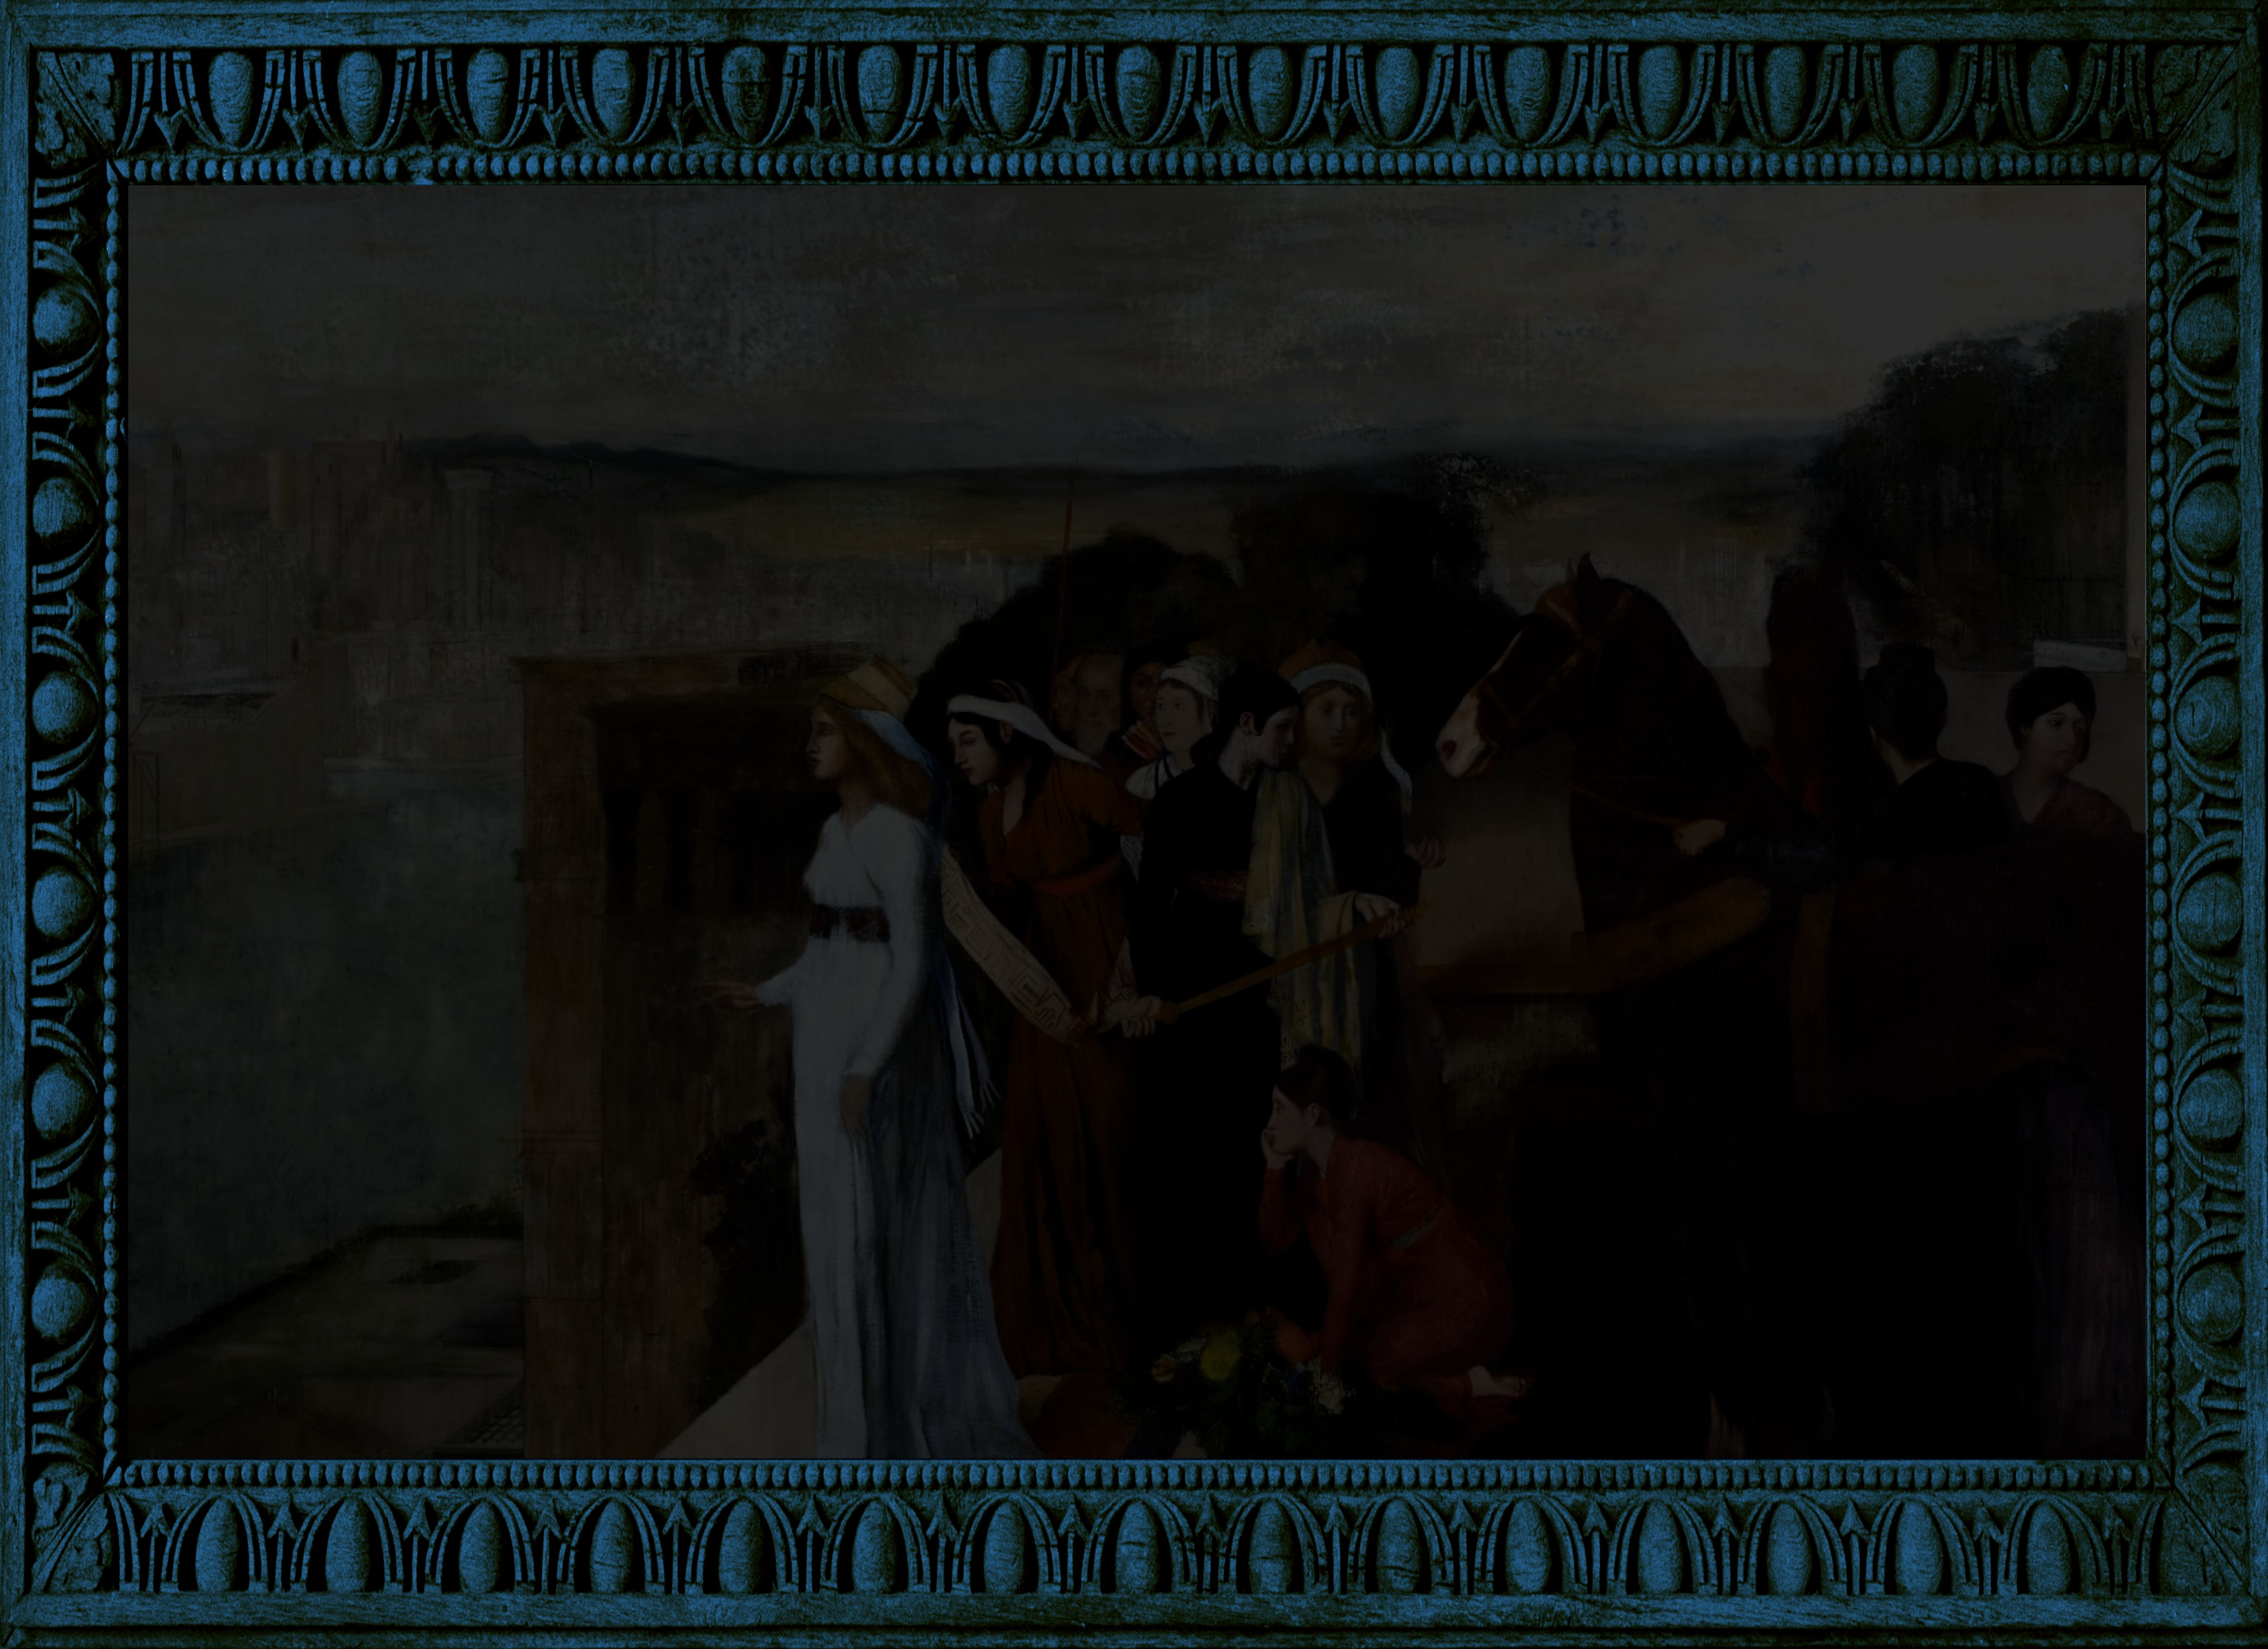
\includegraphics[width=\paperwidth,height=\paperheight]{assyria2.jpeg}}
\renewcommand\thefootnote{{\bfseries\color{White}{\arabic{footnote}}}}
\let\oldfootnote\footnote
    \renewcommand{\footnote}[1]{\oldfootnote{{\bfseries\color{White}#1}}}
\begin{titlepage} % Suppresses headers and footers on the title page
	\centering % Centre everything on the title page
	%\scshape % Use small caps for all text on the title page

	%------------------------------------------------
	%	Title
	%------------------------------------------------
	
	\rule{\textwidth}{1.6pt}\vspace*{-\baselineskip}\vspace*{2pt} % Thick horizontal rule
	\rule{\textwidth}{0.4pt} % Thin horizontal rule
	
	\vspace{1\baselineskip} % Whitespace above the title
	
	{\scshape\Huge La Légende de Sémiramis}
	
	\vspace{1\baselineskip} % Whitespace above the title

	\rule{\textwidth}{0.4pt}\vspace*{-\baselineskip}\vspace{3.2pt} % Thin horizontal rule
	\rule{\textwidth}{1.6pt} % Thick horizontal rule
	
	\vspace{1\baselineskip} % Whitespace after the title block
	
	%------------------------------------------------
	%	Subtitle
	%------------------------------------------------
	
	{\scshape \small Premier Mémoire de Mythologie Comparative 	\vspace{0.5\baselineskip}\\\Large Par François Lenormant} % Subtitle or further description
	
	\vspace*{1\baselineskip} % Whitespace under the subtitle
	
        {\scshape\small Associé de l'Académie Royale de Belgique\\\normalsize Mémoire présenté à la classe des lettres de l'Académie le 8 janvier 1872} % Subtitle or further description
    
	%------------------------------------------------
	%	Editor(s)
	%------------------------------------------------
        \vspace*{\fill}

	\vspace{1\baselineskip}

	{\small\scshape Paris 1873}
	
	{\small\scshape{Maisonneuve et Cie, Libraires. \\ 15, Quai Voltaire}}
	
	\vspace{0.5\baselineskip} % Whitespace after the title block

        \scshape Solar Anamnesis Edition  % Publication year
	
	{\scshape\small CC0 1.0 Universal} % Publisher
\end{titlepage}
\setlength{\parskip}{1mm plus1mm minus1mm}
\clearpage
\tableofcontents
\clearpage
\large
\section*{}
Parmi les légendes relatives à l'ancienne histoire de l'Asie, il n'en est pas qui ait eu une fortune plus brillante que celle de Ninus et de Sémiramis. Elle fut popularisée par Ctésias chez les Grecs, dont le goût pour le merveilleux s'en empara avidement, la trouvant bien plus agréable que les récits \emph{vrais} d'Hérodote. Toute l'antiquité classique y ajouta foi, et depuis la renaissance des lettres les érudits, acceptant implicitement l'idée que cette légende reposait sur un fondement historique véritable, n'ont point songé à en révoquer en doute les faits essentiels, jusqu'au jour où le déchiffrement des textes cunéiformes a révélé d'une manière positive et inattendue que l'histoire de Ninus et de Sémiramis, leurs exploits, leurs immenses conquêtes, n'étaient qu'un tissu de fables puériles, démenti sur tous les points par les faits réels des origines de la monarchie assyrienne.

C'est là un des résultats les plus considérables et les plus positifs qui soient ressortis pour la science historique de l'admirable découverte due au génie pénétrant de Hincks, de sir Henry Rawlinson et de M. J. Oppert, un des faits les mieux établis par les travaux de ces trois fondateurs des études assyriologiques et de ceux qui ont essayé depuis de marcher sur leurs traces. Nous pouvons suivre maintenant la royauté assyrienne dans ses modestes débuts et dans son développement progressif, déterminer l'époque de ses premières conquêtes et celle où elle atteignit l'apogée de sa puissance, et nous n'y voyons rien qui ressemble, même de loin, à cet empire immense, étendu sur toute l'Asie antérieure par le premier de ses rois et se conservant intact pendant une longue suite de siècles, tel qu'il se présentait dans les récits de Ctésias. Mais en même temps l'étude des documents originaux de l'Assyrie, qui n'ont commencé à sortir de terre que dans le dernier demi-siècle et dont on n'est parvenu que depuis bien peu d'années à pénétrer le sens, en nous fournissant des renseignements certains sur la religion commune aux Assyriens et aux Babyloniens, permet de discerner clairement un mythe religieux sous cette légende longtemps considérée comme historique.

Dégager ce mythe des additions et des ornements dont il a été revêtu en pénétrant dans l'histoire, essayer de l'expliquer à la fois par les renseignements que l'on peut dès à présent tirer des textes cunéiformes et par la comparaison des autres religions antiques, tel est l'objet que nous nous sommes proposé dans le présent mémoire, il sera le premier d'une série de dissertations de mythologie comparative dans lesquelles nous étudierons successivement tous les récits assyriens de Ctésias, c'est-à-dire le mythe de Sardanapale et celui de Nannarus et de Parsondas après le mythe de Ninus et de Sémiramis. Nous croyons qu'il nous sera possible de montrer dans ces récits une légende épique d'une nature tout à fait analogue à ce qu'est pour la Perse la légende épique mise en vers et acceptée comme de l'histoire par le poëte Firdoùsi. C'est un enchaînement de récits, à l'origine distincts et purement mythologiques, qui, sous cette forme première, avaient dû prendre naissance en Assyrie même, que la tradition orale du peuple, après la destruction de la monarchie assyrienne et l'oubli des monuments écrits destinés à perpétuer le souvenir de ses annales, avait rassemblés en un seul récit en les transformant en souvenirs nationaux, qu'on regardait comme historiques à la cour de Perse, et cela d'autant plus volontiers que la politique des Achéménides y puisait des arguments en faveur de ses prétentions et de son système. Aussi cette légende épique était-elle devenue pour la chancellerie de Suse l'histoire officielle de la première époque du grand empire asiatique. C'est là que le médecin d'Artaxerxe Mnémon l'avait entendu raconter, et quand même il eût été parfaitement de bonne foi, ce dont il est permis de douter un peu, il était tout naturel qu'il rapportât ces récits à ses compatriotes en croyant leur révéler la vérité sur cette puissante monarchie assyrienne dont le renom était si grand dans tout l'Orient, mais dont les Grecs n'avaient jamais entendu parler que d'une manière très-vague.

\bigskip \centerline{\EightStarTaper} \centerline{\EightStarTaper\EightStarTaper} \bigskip\clearpage
\section{}
\paragraph{}
Nous devons avant tout exposer la légende de Ninus et de Sémiramis afin d'en remettre tous les détails et toutes les circonstances sous les yeux du lecteur. Le récit du mythe, tel qu'il est parvenu jusqu'à nous, doit nécessairement précéder toute tentative d'interprétation. Nous prendrons ici pour guide principal la narration que Diodore de Sicile a extraite de Ctésias, car c'est la plus complète, et d'ailleurs le livre du médecin d'Artaxerxe a été le point de départ de tous les récits analogues qui ont circulé chez les Grecs. Mais nous y ajouterons les circonstances nouvelles qu'y joignent d'autres écrivains, en ayant soin d'en indiquer les sources.

Ninus, fils de Bélus, est donné par la légende comme le premier roi des Assyriens. Amoureux de la guerre et désireux d'acquérir la gloire de fondateur d'un immense empire, il organise une armée composée de jeunes gens d'élite et les prépare par des exercices multipliés à toutes les fatigues et à tous les dangers des combats. Il s'assure l'alliance du roi des Arabes, Ariæus, et renforçant ses troupes par les recrues qu'il tire d'Arabie, il commence ses guerres en assaillant les Babyloniens.

« Leur pays, dit Diodore,\footnote{2., 1.} avait beaucoup de villes bien peuplées ; mais les habitants, inexpérimentés dans l'art de la guerre, furent bientôt vaincus et soumis au tribut. Ninus emmena prisonniers le roi et ses enfants, et les mit à mort. De là il marcha, suivi d'une multitude de soldats, sur l'Arménie, et épouvanta les habitants par le sac de quelques villes. Barzanès, le roi de cette contrée, se voyant hors d'état de résister, alla au-devant de l'ennemi avec des présents, et lui offrit sa soumission. Ninus le traita généreusement, lui laissa son royaume et n'exigea de lui qu'un contingent de troupes auxiliaires. Le roi de Médie, Pharnus, attaqué ensuite, voulut résister ; mais, abandonné des siens, il fut fait prisonnier avec ses sept fils et sa femme, et mis en croix. »

Poursuivant de la même manière le cours de ses succès et n'éprouvant jamais aucun échec, Ninus, en dix-sept ans, subjugua toute l'Asie, à l'exception de la Bactriane et de l'Inde, et joignit aussi à ses États les provinces arrosées par le Nil. Diodore\footnote{2., 2.} énumère ainsi d'après Ctésias les pays et les peuples qui lui obéissaient : l'Égypte, la Phénicie, la Syrie, la Cilicie, la Pamphylie, la Lycie, la Carie, la Phrygie, la Mysie, la Lydie, la Troade, les bords de l'Hellespont, la Propontide, la Bithynie, la Cappadoce, les nations barbares des rivages du Pont-Euxin jusqu'au Tanaïs, les Cadusiens, les Tapyres, l'Hyrcanie, la Drangiane, les Derbices, la Carmanie, les Choromnéens, les Borcaniens, la Parthyène, la Perse, la Susiane et le pays des Caspiens, outre la Babylonie, l'Arménie et la Médie.

Au retour de ces expéditions, et pour donner à ses États une capitale digne de lui, qui surpassât toutes les villes existantes et que la postérité ne pût pas égaler, il construisit sur les bords de l'Euphrate ( ! ! ) Ninive, qu'il appela de son nom. « Cette ville eut la forme d'un quadrilatère oblong. Ses côtés les plus longs avaient 150 stades et les plus courts 90 ; de telle sorte que la totalité de l'enceinte était de 480 stades.\footnote{C'est le chiffre qu'Hérodote (1., 178) assigne à la grande enceinte extérieure de Babylone, et qui, pour cette dernière ville, est exact. Voy. Oppert, \emph{Expédition en Mésopotamie}, t. 1., pp. 220-234.} Les murs avaient 100 pieds de haut et étaient assez larges pour donner passage à trois chars de front. Les tours, au nombre de 1,500, s'élevaient à 200 pieds. Outre les Assyriens, qui formaient la partie la plus nombreuse et la plus puissante de la population, Ninus admit dans sa capitale beaucoup d'étrangers, » et bientôt Ninive devint la plus grande et la plus florissante cité du monde.\footnote{Diod. Sic., 2., 3.}

Ces travaux ne firent pas perdre à Ninus ses goûts guerriers ; sa nouvelle ville achevée, il entreprit la conquête de la Bactriane, qu'il avait déjà vainement tentée. C'est dans le cours de cette guerre que se montra pour la première fois Sémiramis, qui allait bientôt attacher à son nom une si grande célébrité. « Il y a en Syrie, dit Diodore, empruntant les propres paroles de Ctésias, une ville nommée Ascalon, près de laquelle est un étang grand et profond, rempli de poissons. A côté de cet étang s'élève le temple d'une déesse fameuse, que les Syriens appellent Dercéto et représentent avec un buste de femme sur un corps de poisson. Les plus instruits des indigènes racontent qu'Aphrodite, irritée contre cette déesse, lui inspira un violent amour pour un beau et jeune ministre de son temple. Dans les embrassements de ce jeune Syrien, Dercéto devint mère d'une fille, mais bientôt, rougissant de sa faute, elle fit périr son amant et exposa sa fille dans un lieu désert au milieu de rochers. Elle-même, poussée par la honte et par la douleur, se jeta dans l'étang, où elle se transforma en poisson ; aussi, depuis lors, les Syriens s'abstiennent-ils de manger du poisson et rendent-ils à ces animaux des honneurs divins. Cependant de nombreuses colombes nichaient autour du lieu où l'enfant avait été exposé ; elles le nourrirent et lui sauvèrent la vie d'une manière miraculeuse et divine, les unes le réchauffant en l'enveloppant de leurs ailes, les autres apportant dans leur bec et faisant dégoutter sur ses lèvres du lait enlevé aux bergeries voisines. Puis, quand l'enfant eut atteint l'âge d'un an et commença à avoir besoin d'une nourriture plus solide, ce furent des fromages que les colombes dérobèrent pour les lui apporter. Les bergers finirent par s'en apercevoir, et ayant fait le guet, suivirent les colombes jusqu'au lieu où ils trouvèrent la petite fille, admirable de beauté. L'ayant apportée dans leurs cabanes, ils la présentèrent à l'intendant des propriétés royales, nommé Simmas. Celui-ci, n'ayant pas d'enfants, l'éleva comme sa fille et la nomma Sémiramis, du mot qui, dans la langue syrienne, signifie colombe ; et depuis ce temps, les Syriens honorèrent les colombes comme des divinites.\footnote{Diod. Sic., 2., 4 ; cf. Lucian., \emph{De dea Syr.}, 14 ; Eratosthen., \emph{Catasterism.}, 38 ; Athenagor., \emph{Legat. pro Christian.}, 26 ; Anonym., \emph{De mulier}., dans Heeren, \emph{Bibliothek der alt. Liter. u. Kunst.}, part. 6., p. 9.} »

Après avoir grandi dans la maison de Simmas, Sémiramis fut épousée pour sa beauté par le gouverneur de Syrie, nommé Ménonès. --- Les autres auteurs qui ont également emprunté leurs données à Ctésias, écrivent Onnès ou Oannès, et cette leçon paraît plus exacte.\footnote{Nicol. Damasc., \emph{ap.} C. Müller, \emph{Fragment. historic. græc.}, t. 3., p. 356 ; et l'Anonyme auteur du traité \emph{De mulieribus}.} --- Elle ne tarda pas à prendre un empire absolu sur l'esprit de son mari, et elle le suivit à l'armée royale dans la guerre de Bactriane. Ninus avait emmené dans cette expédition 1,700,000 fantassins, 210,000 cavaliers et 10,600 chars armés de faux.\footnote{Diod. Sic., 2., 5.}

Un acte de bravoure, exceptionnel pour son sexe, valut à Sémiramis d'être distinguée par Ninus et de devenir reine. Vaincu d'abord par les Bactriens dans une bataille où ils perdirent 100,000 hommes, les Assyriens avaient repris l'avantage ; devenus maîtres des principales villes du pays, ils assiégeaient la capitale, où s'était retiré le roi Oxyartès. --- D'autres auteurs font de Zoroastre le roi enfermé dans Bactres.\footnote{Cephalion, \emph{ap.} Euseb., \emph{Arm. Chron.}, p. 41, ed. Mai, \emph{et ap.} Mos. Choren., 1., 17 ; Just., 1., 1.} --- Mais le siége trainait en longueur, lorsque Sémiramis, travestie en guerrier, trouva moyen d'escalader la forteresse, et, par un signal élevé sur le mur, avertit de son succès les troupes de Ninus, qui emportèrent la place. Ninus, émerveillé de tant de bravoure et de la beauté de Sémiramis, l'enleva à Ménonès et en fit son épouse. Ménonès se pendit de désespoir.\footnote{Diod. Sic., 2., 6.}

Peu de temps après, Ninus, ayant eu de Sémiramis un fils nommé Ninyas, mourut, et la laissa souveraine de l'empire.\footnote{\emph{Ibid.}, 7.} Suivant d'autres écrivains, il se retira en Crète, lui laissant le champ libre en Assyrie.\footnote{Mos. Choren., 1., 16.} Une troisième version de la légende raconte encore différemment l'élévation de Sémiramis. Elle en fait une courtisane introduite à cause de sa rare beauté comme concubine dans le harem de Ninus. Lois de la célébration des Sacées,\footnote{Sur cette fête célèbre, voy. notre \emph{Essai de commentaire des fragments cosmogoniques de Bérose}, pp. 167-174.} Sémiramis obtient de s'asseoir sur le trône comme reine de la fête ; alors elle donne l'ordre de jeter le monarque en prison et de le mettre à mort ; et c'est ainsi qu'elle s'empare du pouvoir.\footnote{Diod. Sic., 2., 20 ; Ælian., \emph{Var. hist.}, 7., 1.}

Ninus fut enterré sons une pyramide haute de 9 stades et large de 10 à la base, dans le palais de Ninive. Quant à Sémiramis, une fois eu possession de la puissance suprême, elle donna l'essor à son génie naturellement entreprenant. Jalouse de surpasser la gloire de son époux, elle conçut le dessein de bâtir sur le bas Euphrate une ville immense ; ce fut Babylone, qui n'existait pas jusqu'alors.\footnote{Diod. Sic., 2., 7.}

Ctésias rapportait à Sémiramis, conformément à la légende, toutes les grandes constructions de Babylone, les murs, auxquels il donnait la hauteur fabuleuse de 50 orgyies et une largeur suffisante pour faire passer six chars de front,\footnote{\emph{Ibid.}} les quais et le pont de l'Euphrate, les deux palais, dont il donnait une description très-exacte,\footnote{\emph{Ibid.}, 8.} le grand lac artificiel situé en amont de la ville et dans lequel on avait détourné l'Euphrate pendant la construction du tunnel qui reliait les deux palais par-dessous le fleuve, enfin la pyramide regardée comme le tombeau de Bélus.\footnote{\emph{Ibid.}, 9.} Cependant il reconnaissait que les fameux jardins suspendus « n'étaient pas l'œuvre de Sémiramis, mais d'un roi syrien postérieur, qui les avait élevés pour une de ses femmes.\footnote{\emph{Ibid.}, 10.} » Mais il racontait que Sémiramis avait encore construit de nombreuses villes destinées à servir de marchés le long de l'Euphrate et du Tigre, et qu'elle avait fait apporter par eau, des montagnes de l'Arménie, un obélisque prodigieux, haut de 130 pieds et large de 25, qu'elle avait dressé à la porte de Babylone.\footnote{\emph{Ibid.}, 11.} Justin parle aussi de la construction de Babylone par cette reine fameuse.\footnote{Justin., 1., 2.}

Sémiramis, après avoir achevé ces ouvrages dans la Babylonie, entreprit une expédition contre les Mèdes, qui s'étaient révoltés. Elle soumit de nouveau leur pays et y laissa des monuments immortels de son passage. Arrivée au pied du mont Bagistan, elle y créa un \emph{paradis} merveilleux, et sur une des parois de la montagne, formée de rochers taillés à pie d'une hauteur effrayante, elle fit sculpter son image entourée de celle de cent de ses gardes, avec une inscription racontant ses exploits. Auprès de Chavon, elle fit établir un autre \emph{paradis} entourant un rocher de dimensions extraordinaires, et elle s'y arrêta longtemps, se livrant à tous les plaisirs, tandis que son armée campait aux environs. Elle ouvrit une route taillée dans le roc au travers du mont Zarcæus. Diodore lui attribue aussi la fondation d'Ecbatane et de son palais. Comme la ville manquait d'eau el qu'il n'y avait aucune source dans le voisinage, elle amena à grands frais et à l'aide de travaux prodigieux une eau pure et abondante dans tous les quartiers. Pour cela elle perça le mont Oronte et y creusa un tunnel de 15 pieds de largeur sur 40 de hauteur, qui communiquait avec un lac situé de l'autre côté de la montagne.\footnote{Diod. Sic., 2., 13.}

De la Médie, Sémiramis se dirigea vers la Perse et parcourut toutes les autres contrées qu'elle possédait dans l'Asie. En Arménie elle éleva, près du lac de Van, une ville qui fut appelée Sémiramocerte, avec un palais immense.\footnote{Mos. Choren., 1., 16.} Partout où elle allait, elle perçait les montagnes, brisait les rochers, pratiquait de grandes et belles routes. Dans les plaines, elle érigeait des tertres qui servaient de tombeaux à ses généraux morts pendant l'expédition.\footnote{Diod. Sic., 2. 14.} D'autres disaient qu'elle les avait élevés en prévision d'un déluge futur.\footnote{Syncell., p. 64, C.} Mais une version beaucoup plus répandue en faisait les tombeaux de ses amants mis à mort.\footnote{Ctes. \emph{ap.} Johan. Antioch., Cramer, \emph{Anced. Paris}, t. 2, p. 386 ; Syncell., p. 64, C.} La légende, dans toutes ses formes, était en effet unanime pour attribuer à Sémiramis de nombreuses débauches. Ayant toujours refusé, disait-on, de contracter un nouveau mariage légitime, elle prenait pour ses amants les plus beaux hommes de son armée, et quand son caprice était une fois satisfait, elle les faisait tuer.\footnote{Diod. Sic., 2., 13.} On allait plus loin, et on lui attribuait d'étranges amours avec un cheval, pour lequel elle s'était enflammée d'une passion violente.\footnote{Jub. \emph{ap.} Plin., \emph{Hist. nat.}, 8., 42, 64.}

L'Asie parcourue, Sémiramis se rendit en Egypte, car ce pays faisait aussi partie de son empire. De là elle alla visiter l'oracle d'Ammon, qui lui prédit qu'elle disparaîtrait miraculeusement du milieu des hommes et serait honorée comme une divinité, après que son fils Ninyas aurait conspiré contre sa vie. Elle fit ensuite la conquête de l'Éthiopie, dont elle admira les fabuleuses merveilles.\footnote{Diod. Sic., 2., 14.}

Mais la soumission de l'Éthiopie n'avait pas demandé de combats, et Sémiramis brûlait de l'ambition d'ajouter la gloire militaire à toute sa renommée. Elle résolut donc d'entreprendre la conquête de l'Inde, dont les immenses richesses excitaient d'ailleurs sa convoitise. Stabrobatis, roi des Indiens, averti des préparatifs inouïs de la reine d'Assyrie, mit sur pied des forces considérables, puis défia Sémiramis elle-même, dans une lettre où il lui reprochait ses débauches, et la menaçait de la mettre en croix s'il était vainqueur. Sémiramis n'en attaqua pas moins le monarque indien, et parvint d'abord à forcer le passage de l'Indus. Mais dans la grande bataille qui s'ensuivit, les éléphants de Stabrobatis lui assurèrent la victoire. La reine elle-même fut blessée, son armée mise en fuite et détruite aux deux tiers ; mais les Indiens, par l'ordre des dieux, ne la poursuivirent pas au-delà du fleuve.\footnote{\emph{Ibid.}, 16-20.} Quand Mégasthène, ambassadeur de Séleucus à la cour de Pàtalipoutra (la Palibothra des Grecs), consulta les chroniques et les traditions nationales des Indiens, il n'y trouva aucune trace de l'expédition de Sémiramis. Mais n'osant pas révoquer en doute l'existence de cette reine, à laquelle tous les Grecs croyaient fermement de son temps, il supposa qu'elle avait dû mourir avant de pouvoir réaliser son projet d'attaque contre cette partie lointaine de l'Asie.\footnote{Strab., 15., p. 687 ; Arrian., \emph{Indie.}, 5, 4.}

C'est au retour de la campagne si tristement terminée dans l'Inde, qu'on racontait que Sémiramis avait été en butte à une conspiration des deux fils issus de son mariage avec Oannès, lesquels sont nommés Hyapatès et Hydaspès.\footnote{Diod. Sic., 2., 5.} Révoltés des désordres de leur mère et excités par l'eunuque Satibaras, les deux jeunes gens avaient résolu de l'assassiner ; prévenue, Sémiramis les fit mettre à mort.\footnote{Nicol. Damasc. \emph{ap.} C. Müller, \emph{Fragm. historic. græc.}, t. 3, p. 356 ; Cephalion \emph{ap.} Euseb., \emph{Armen. chron.}, p. 41, ed. Mai, \emph{et ap.} Mos. Choren., 1., 17.}

Au reste, à la suite de cet échec, elle rentra dans ses États, d'où elle ne sortit plus. Elle poursuivit l'exécution de ses vastes travaux ; et telles furent l'activité et la renommée de cette reine qu'après elle, suivant Strabon, tout grand ouvrage en Asie lui fut attribué par la voix populaire.\footnote{Strab., 16., p. 737.} Alexandre trouva, raconte-t-on, son nom inscrit sur les frontières de la Scythie, alors considérée comme la borne du monde habité. C'est cette inscription dont le texte prétendu nous a été conservé par Polyen\footnote{\emph{Stratagem.}, 8., 26.} et dans laquelle Sémiramis, parlant d'elle-même, se serait exprimée ainsi : « La nature m'a donné le corps d'une femme, mais mes actions m'ont égalée au plus vaillant des hommes. J'ai régi l'empire de Ninus qui vers l'Orient touche au fleuve Hinamanès (évidemment celui que la plupart des géographes anciens nomment Etymander), vers le sud au pays de l'encens et de la myrrhe, vers le nord aux Saces et aux Sogdiens. Avant moi, aucun Assyrien n'avait vu de mers ; j'en ai vu quatre, que personne n'abordait, tant elles étaient éloignées. J'ai contraint les fleuves de couler où je voulais, et je ne l'ai voulu qu'aux lieux où ils étaient utiles : j'ai rendu féconde la terre stérile en l'arrosant de mes fleuves. J'ai élevé des forteresses inexpugnables, j'ai percé avec le fer des routes à travers les rochers impraticables. J'ai frayé à mes chariots des chemins que les bêtes féroces elles-mêmes n'avaient pas parcourus. Et au milieu de ces occupations, j'ai trouvé du temps pour mes plaisirs et pour mes amours. »

Cependant, ayant appris que son fils Ninyas lui tendait des embûches, Sémiramis se souvint des prédictions de l'oracle d'Ammon et prit le parti d'abdiquer. Loin de punir le conspirateur, elle lui remit l'empire, ordonna à tous les gouverneurs d'obéir au nouveau souverain, puis elle disparut, changée en colombe, au milieu d'un vol de ces oiseaux. Les Assyriens en firent une déesse et rendirent, à cause d'elle, des honneurs divins à la colombe.\footnote{Diod. Sic., 2., 20.} D'autres récits la font tuer par son fils Ninyas.\footnote{Cephalion \emph{ap.} Euseb., \emph{Armen. chron.}, p. 41, ed. Mai, \emph{et ap.} Mos. Choren., 1., 17.} On disait même que celui-ci l'avait frappée dans son horreur pour la passion incestueuse dont elle le poursuivait.\footnote{Justin., 1., 2.} Quant à la tradition arménienne, elle avait pris un caractère tout local. Elle prétendait que Sémiramis résidait à Sémiramocerte, sur le lac de Van, quand Zoroastre, qu'elle avait institué satrape d'Assyrie, se révolta et marcha contre elle. Elle s'enfuit alors presque seule dans les montagnes de l'Arménie, où elle fut tuée par son fils Ninyas.\footnote{Mos. Choren., 1., 16.}

La chronologie rattachée à ces récits n'est pas moins fabuleuse que la légende elle-même. Elle place Ninus et Sémiramis, avec leurs immenses conquêtes et leur empire qui embrasse toute l'Asie, dans un temps où il n'était pas encore même question d'une monarchie assyrienne.\footnote{Nous ne pouvons pas ici donner incidemment un récit des premiers temps de la royauté assyrienne, tels que les documents indigènes nous mettent à même de les reconstituer aujourd'hui, en nous faisant connaître les traits principaux de cette antique histoire. Nous nous bornerons donc à renvoyer le lecteur aux deux résumés les plus récents qui aient été donnés de l'état actuel de la science sur ce point : celui de M. Smith dans les derniers numéros de l'année 1868 de la \emph{Zeitschrift für Ægyptische Sprache und Alterthumskunde} de M. Lepsius ; et celui de notre \emph{Recueil de l'histoire ancienne de l'Orient}, 3\textsuperscript{e} édition (1869), t. 2., pp. 55 et suiv.\\\hspace*{5mm}Rappelons seulement qu'un peu avant l'année 1800 av. J.-C. --- 701 ans avant \emph{Tuklati-pal-as'ar} 1\textsuperscript{er}, d'après le témoignage formel du prisme de ce dernier prince (col. 7, l. 60-73 : \emph{Cuneiform inscriptions of Western Asia}, t. 1., pl. 15) --- il n'y avait pas encore de rois d'Assyrie, mais des pontifes (\emph{patesi}) du dieu \emph{As's'ur} régnant sur la ville d'\emph{Al-As's'ur}, la \<'lsr> de la Bible, aujourd'hui Kalah-Scherghât.\\\hspace*{5mm}Le plus ancien roi d'Assyrie proprement dit, \emph{s'ar As's'ur}, que nous connaissions vivait environ 1400 ans avant l'ère chrétienne. Babylone fut soumise à la suzeraineté ninivite, tout en gardant ses rois propres, par \emph{Tuklati-\d{S}amdan} 1\textsuperscript{er}, vers 1270 seulement. Et ceci coïncide fort exactement avec ce que dit Hérodote (1., 95) que la puissance des Assyriens en Asie commença 520 ans avant l'époque où les Mèdes se rendirent indépendants. Nous nous sommes, en effet, efforcé de prouver ailleurs (dons la première de nos \emph{Lettres assyriologiques}) que ce dernier événement devait être placé entre 750 et 745 av. J.-C.\\\hspace*{5mm}\emph{Adar-pal-as'ar}, dont il est dit (\emph{Cuneif. inscr. of West. As.}, t. 1., pl. 15, col. 7, l. 56-59) que « il organisa le pays d'Assyrie ... et institua le premier les armées d'Assyrie, » est voisin de 1210, et les grandes conquêtes débutent seulement au douzième siècle, encore avec un développement bien loin d'approcher de celui qu'elles reçurent de la fin du dixième siècle au commencement du septième.} Ctésias comptait 33 règnes et 1306 ans de durée entre Ninus et Sardanapale,\footnote{Diod. Sic., 2., 21 et 28 ; Syncell., p. 359, C ; Agathias, 2., 25 ; Augustin, \emph{De civit. Dei}, 18., 21.} et plaçait le détrônement de ce dernier roi par Arbace en 876 avant notre ère\footnote{Diod. Sic., 2., 32-34 ; Agathias, 2., 25.} ; cela reporte Ninus en 2182 et concorde exactement avec l'autre affirmation du même écrivain qu'il était de mille ans antérieur à la prise de Troie.\footnote{Diod. Sic., 2., 28.} Velleius Paterculus\footnote{1., 6, 6.} et Justin\footnote{1., 3.} donnent le même calcul emprunté à la même source. Pour Castor de Rhodes, la chute de Ninive est de 843 avant notre ère et l'avènement de Ninus se place 1280 ans plus tôt,\footnote{\emph{Ap.} Euseb., \emph{Armen. chron.}, p. 36, ed. Mai.} c'est-à-dire en 2123. Quant à Céphalion, Sardanapale est, dans son système, inscrit en 1150 et la durée de l'empire depuis Ninus de 1013 ans,\footnote{Euseb., \emph{Armen. chron.}, p. 41-44, ed. Mai ; Syncell., pp. 167 et 168.} ce qui reporte le fondateur en 2163. On voit que tous ces calculs reviennent, à bien peu de chose près, à la même date, qui était évidemment donnée par la légende et qui en avait le caractère fantastique.

\bigskip \centerline{\EightStarTaper} \centerline{\EightStarTaper\EightStarTaper} \bigskip\clearpage
\section{}
\paragraph{}
Il est facile de discerner deux éléments, l'un épique et l'autre religieux, dans la formation de cette célèbre légende, qui, nous l'avons déjà dit tout à l'heure, avait surtout pris un grand développement sous les Perses et que leur politique exploitait à leur profit, mais qui avait également cours chez les peuples sémitiques, et dont le fond premier, nous l'avons dit aussi et nous allons essayer de le démontrer dans un instant, devait ne pas être étranger aux Assyriens eux-mêmes, car il se rattachait à des mythes de leur religion.

Au point de vue des souvenirs historiques confondus et groupés dans un seul ensemble par l'imagination populaire, et transformés en épopée, Ninus, son nom même l'indique suffisamment, est le héros éponyme de la ville de Ninive, la personnification de cette ville et de sa puissance ; sous son nom les récits de la tradition orale ont groupé tous les exploits, toutes les conquêtes des rois des différentes dynasties assyriennes, et même, car ces récits amplifient toujours, des conquêtes que n'a jamais faites aucun monarque de Ninive, comme celle de la Bactriane, et dans une autre direction celle des provinces occidentales de l'Asie Mineure. De même que les expéditions militaires ont été réunies autour du nom de Ninus, bien qu'on en ait aussi attribué à Sémiramis, la légende a surtout gratifié cette reine fabuleuse de la gloire de tous les travaux utiles ou gigantesques exécutés aux époques les plus diverses par des souverains asiatiques, quelle qu'en fût l'origine.\footnote{Voy. notre \emph{Manuel d'histoire ancienne de l'Orient}, 3\textsuperscript{e} édit., t. 2., p. 50 et suiv.} Elle lui a attribué toutes les constructions de Babylone,\footnote{Ce qui put y contribuer pour une certaine part, c'est que des travaux considérables et d'une grande utilité avaient été réellement exécutés à Babylone, vers la fin du neuvième siècle avant notre ère, par une reine qu'Hérodote (1., 184) appelle Sémiramis et qu'il place fort exactement un siècle et demi avant Nitocris, la femme de son Labynète 1\textsuperscript{er}, c'est-à-dire de \emph{Nabu-bal-usur} (Nabopolassar), roi de Babylone. « Sémiramis, dit le père de l'histoire, fit faire ces digues magnifiques qui retiennent l'Euphrate dans son lit et l'empêchent d'inonder la campagne autour de Babylone. » C'est la seule Sémiramis historique, et on l'a reconnue avec certitude dans la reine \emph{Sammu-ramat}, femme du roi d'Assyrie \emph{Bin-nirari} 3, que mentionne l'inscription de la statue du dieu \emph{Nabu} découverte par M. Loftus à Nimroud et actuellement conservée au Musée Britannique (\emph{Cuneif. inscr. of West. As.}, t. 1, pl. 35, n° 2 ; voy. la représentation de la statue elle-même dans George Rawlinson, \emph{The five great monarchies of the ancient eastern world}, 1re édit., t. 1., p. 179). Cette reine parait avoir été une princesse babylonienne de naissance, épousée par le monarque assyrien, qui aura régné de nom à Babylone en même temps que son mari à Ninive, et que les Babyloniens auront plus tard enregistrée seule dans leurs annales nationales. Voy. notre \emph{Manuel d'histoire ancienne de l'Orient}, 3\textsuperscript{e} édit., t. 2., p. 76.} depuis celle de la pyramide de Bel, que les Babyloniens eux-mêmes rapportaient « au plus ancien roi, » jusqu'à celles du temps de \emph{Nabu-kudurri-usur} et de ses successeurs ; elle a placé de même sous son nom les travaux du roi Déjocès à Ecbatane,\footnote{Hérodote, 1., 98.} et l'exécution des grandioses sculptures du mont Bagistan dans la Médie (aujourd'hui Behistoun), qui datent du règne de Darius fils d'Hystaspe.\footnote{Il faut cependant remarquer que Ker-Porter (\emph{Travels}, t. 2., p. 151 et suiv.) signale sur le rocher de Behistoun, et dans une position plus basse, un second bas-relief, dont il trouvait le style analogue à celui du grand bas-relief de Darius, mais presque effacé et difficile à distinguer. On serait tenté de croire que c'est à cette sculpture que faisait allusion la légende recueillie par Ctésias, car on a quelque peine à admettre que l'origine d'un monument de Darius fils d'Hystaspe fût déjà complétement oubliée du temps d'Artaxerxe Mnémon. Mais aucun autre voyageur ne parle de ce second bas-relief et l'on n'en voit pas de trace dans la grande vue du rocher de Behistoun que MM. Coste et Flandin ont donnée dans leur ouvrage sur la \emph{Perse ancienne}.}

C'est là le côté non assyrien de la légende sous la forme où Ctésias l'a recueillie. Ce sont les broderies poétiques que l'imagination des peuples voisins a superposées au vieux mythe religieux venu de l'Assyrie, en y greffant les souvenirs gigantesques, mais confus et sans chronologie, que leur avait laissés la puissance du grand empire qui les avait si longtemps tenus sous le joug. En effet, si les Assyriens avaient des héros éponymes à l'origine de leurs cités et des légendes épiques sur les premiers temps de leur nation,\footnote{Nous trouvons un précieux débris de ces légendes assyriennes de héros éponymes dans un passage d'Abydène qui nous a été conservé par Eusèbe (\emph{Armen. chron.}, p. 36, ed. Mai) : \emph{Fuit Ninus Arbeli, Chaali, Arbeli, Anebi, Babii, Beli regis Assyriorum}. Le même passage est reproduit par Moïse de Khorène (1., 4) : \emph{Ninus ortus Arbelo, Chaealus Arbelo ; is Anebi, is Babio, is Belo}.\\\hspace*{5mm}Quelques remarques sur l'origine première de ces données sont ici nécessaires. Abydène parait avoir suivi dans son livre la marche suivante. Après avoir exposé l'histoire de la Babylonie en résumant Bérose jusqu'au règne d'Alexandre le Grand, il racontait l'histoire des Assyriens conformément au système de Ctésias, sur lequel les Grecs n'élevaient aucun doute, en la commençant à Ninus et en la finissant à Sardanapale. C'est ce qui ressort du témoignage formel d'Eusèbe (\emph{Armen. chron.}, p. 36, éd. Mai) : \emph{Abydeni de regno Assyriorum. Chaldaei regionis suae reges ab Aloro usque ad Alexandrum hoc pacto enumerant. Nini quidem et Samiramidis nullam rationem habent. His autem dictis ita suam historiam exorditur.} Suit la phrase que nous venons de citer sur la généalogie de Ninus, puis le texte reprend. \emph{Deinde adcurate reges enumerat a Nino et a Samiramide ad Sardanapallum, qui omnium extremus fuit : a quo ad primam Olympiadem sexaginta et septem anni putantur. De Assyriorum regno hac diligentia scripsit Abydenus. Nihilominus et Castor primo libro summarii chronicorum eadem plane ad literam narrat de regno Assyriorum.} Il semblerait, du reste, d'après la phrase (\emph{Chaldaei}) \emph{Nini et Samiramidis nullam rationem habent}, qu'Abydène faisait ressortir la contradiction des deux récits de Bérose et de Ctésias, trop frappante pour ne pas être remarquée de quiconque essayait de les mettre en parallèle. Pour la date de Sardanapale il suivait le même système que Castor de Rhodes, soit qu'il la lui eût empruntée, soit que Castor l'ait, au contraire, copiée dans Abydène. Mais il s'en écartait considérablement pour le reste de l'histoire, ainsi qu'on peut s'en convaincre en étudiant l'extrait de Castor donné par Eusèbe (\emph{Armen. chron.}, p. 36, ed. Mai) immédiatement après celui d'Abydène et la liste des rois d'Assyrie dans les \emph{Excerpta barbara} publiés par Scaliger (\emph{De emend. tempor.}, p. 74), liste qui procède certainement de Castor par l'intermédiaire de Jules l'Africain. Castor faisait suivre immédiatement Bélus par Ninus, tandis qu'Abydène plaçait, comme on vient de le voir, plusieurs noms dans l'intervalle. Castor ne finissait pas la liste royale avec Sardanapale, mais lui donnait un successeur, Ninus 2 ; Abydène, conformément à Ctésias, présentait Sardanapale comme le dernier de tous, \emph{omnium extremus}, et faisait coïncider la destruction de l'empire avec sa mort.\\\hspace*{5mm}Mais d'où pouvait provenir la série de rois qui nous a conduit à nous occuper ici du livre d'Abydène et que cet auteur insérait entre Bélus et Ninus ? Or n'est certainement pas de Ctésias, puisqu'aucun autre des auteurs qui ont parlé de l'histoire d'Assyrie d'après le médecin d'Artaxerxe ne connaît ces rois. D'ailleurs cette courte liste offre un tout autre caractère que la longue liste de Ctésias, au commencement de laquelle Abydène l'avait artificiellement greffée.\\\hspace*{5mm}Le canon des rois assyriens de Ctésias, que nous ne connaissons, du reste, qu'un peu altéré, puisque les deux versions d'Eusèbe et du Syncelle ne s'accordent pas de tous points et contiennent trois princes de plus que le nombre indiqué par Diodore, le canon de Ctésias se compose de noms purement de fantaisie. Les uns sont iraniens et ont certainement été copiés par Ctésias dans les chroniques perses qu'il consultait, comme \emph{Arius} (4\textsuperscript{e}), \emph{Aralius} (5\textsuperscript{e}), \emph{Xerxes} (6\textsuperscript{e}), \emph{Armamithres} (7), \emph{Mithræus} (25\textsuperscript{e}) ; d'autres, en bien petit nombre, qui ont dû être empruntés aux mêmes chroniques, ont une certaine physionomie assyrienne et proviennent probablement de traditions populaires, comme \emph{Sardanapallus} (36\textsuperscript{e}), qui rappelle \emph{As's'ur-bani-pal}. Nous avons été longtemps porte à rattacher à cette catégorie \emph{Belochus} (18\textsuperscript{e}), à qui nous trouvions beaucoup d'analogie avec un nom que nous lisions alors \emph{Bin-liχχus'} ; mais le rapprochement n'est plus possible aujourd'hui que des exemples positifs établissent pour ce nom royal la lecture \emph{Bin-nirari}. Il est à remarquer que les rares noms auxquels nous venons de faire allusion ont précisément une analogie frappante avec ceux de conquérants assyriens qui eurent affaire aux peuples aryens et durent par conséquent laisser chez eux un souvenir ; seulement ils sont mis tout à fait en dehors de leur vraie place historique. Mais à côté nous voyons des noms purement grecs qu'il est bien difficile de ne pas croire inventés par Ctésias lui-même pour remplir les lacunes des chroniques perses ; tels sont ceux d'\emph{Amyntas} (17\textsuperscript{e}), \emph{Lamprides} (20\textsuperscript{e}), \emph{Panyas} (23\textsuperscript{e}), \emph{Laosthenes} (31\textsuperscript{e}), \emph{Peritiades} (32\textsuperscript{e}). Une dernière catégorie, surtout dans la dernière partie de la liste, est formée de noms géographiques, tous empruntés à des fleuves ou à des canaux de la Babylonie, \emph{Dercylus} (29\textsuperscript{e}), \emph{Ophratæus} (33\textsuperscript{e}), \emph{Ophratanes} (34\textsuperscript{e}), \emph{Acragunes} (35\textsuperscript{e}), sans compter les noms pris à l'histoire d'Égypte, on ne sait pourquoi, comme \emph{Sethos} (10\textsuperscript{e} suivant le Syncelle) et \emph{Lampares} (22\textsuperscript{e}). Ce que cette liste offre de plus frappant, c'est qu'elle ne renferme pas un seul élément historique réel, confirmé par les monuments.\\\hspace*{5mm}Dans le fragment que nous avons cité, au contraire, nous trouvons une série d'éponymes de cités véritablement assyriennes, caractère que ne présente aucun des noms de Ctésias ; ces noms sont rangés dans un ordre géographique régulier, et par leur ordre même ils expriment un fait historique véritable, qu'atteste en termes formels le chapitre 10 de la Genèse, d'accord avec tous les monuments, la marche de la civilisation remontant le cours du Tigre depuis Babylone jusqu'à Ninive. Une donnée historique aussi exacte et aussi précise, et qui contraste si nettement avec les fables perses recueillies par Ctésias, ne peut manquer d'avoir eu une source réellement assyrienne ; elle a été puisée dans les documents indigènes, et en dehors de Bérose, aucun écrivain de la littérature grecque n'a été aussi bien informé. Or, Abydène travaillait d'après deux auteurs, Bérose et Ctésias. Quand nous rencontrons chez lui un renseignement sur les origines de l'Assyrie qui n'appartient certainement pas à Ctésias et qui se distingue de ses fables par un caractère de tradition réellement indigène, nous sommes en droit d'en attribuer l'origine à Bérose, d'autant plus que l'historien de la Chaldée semble avoir mentionné à son point de vue Ninus et Sémiramis (Euseb. \emph{Armen. chron.}, p. 18. ed. Mai) et par conséquent avoir fait, au moment où les Assyriens apparaissaient dans les annales de Babylone, un retour en arrière sur leurs traditions légendaires et les débuts de leurs annales.\\\hspace*{5mm}C'est à M. Oppert qu'appartient le mérite d'avoir reconnu, dès le \emph{Rapport ou ministre de l'instruction publique} où il a exposé (en 1856) les premiers résultats de ses travaux, le véritable caractère de la petite liste que nous avons sous les yeux et d'y avoir montré d'une manière certaine des noms de villes disposés dans un ordre géographique régulier correspondant à une réalité historique. Mais avant lui, Ottfried Müller l'avait déjà soupçonné, dans sa dissertation intitulée : \emph{Sandon und Sardanapal}, qui a paru au tome 3 de la première série du \emph{Rheinisches Museum für Philologie}. Au reste, il suffit de jeter les yeux sur cette liste, avec les connaissances que nous commençons à avoir sur la géographie antique de la Babylonie et de l'Assyrie, pour y reconnaître des noms de villes à peine altérés par leur hellénisation et par les copies successives ; quant à la régularité de l'ordonnance géographique remontant du sud au nord, elle est aussi saisissante dès que l'on corrige l'erreur manifeste de la répétition du nom d'\emph{Ar-belus} dans Eusèbe et dons Moïse de Khorène, d'après le Syncelle (pp. 151, 154 et 155) qui a inséré de la façon la plus bizarre cette liste de rois, très-exactement reproduite, mais retournée dans l'ordre inverse, entre le vingt-septième et le vingt-huitième nom du canon de Ctésias.\\\hspace*{5mm}Voici en effet de quelle façon le document que nous considérons comme emprunté à Bérose par Abydène marque, au moyen des éponymes des principales villes, les étapes de la civilisation remontant, avec la domination du peuple des Nemrodites ou Kouschites (voy. notre \emph{Essai de commentaire des fragments cosmogoniques de Bérose}, p. 43), de la Babylonie dans l'Assyrie.\begin{table}[H]
    \centering
    \tiny
    \bfseries
    \begin{tabular}{l l}
    \hline
        Noms des Rois Éponymes: & Noms Assyriens des Villes: \\\hline
        Babius. & \emph{Babilu}. \\
        Anebus. & \emph{Nipur}. \\
        Chaalus ou Chalaüs. & \emph{Kalaχ}. \\
        Arbelus. & \emph{Arbait}. \\
        Ninus. & \emph{Ninua}. \\
    \end{tabular}
\end{table}Le parallélisme des deux ordres de noms est assez frappant pour n'avoir pas besoin d'autre commentaire. Quant à Bélus, c'est le dieu \emph{Bel}, qui figure à bon droit en tête, avant le héros éponyme de Babylone, car la tradition nationale, attestée par les monuments et enregistrée par Bérose (Euseb., \emph{Armen. chron.}, p. 27, ed. Mai ; \emph{Praepar. Evan.}, 9., 41) lui attribuait la fondation de cette ville.\\\hspace*{5mm}Que les Assyriens, dont l'histoire positive commençait fort tard en comparaison de celle des Babyloniens, aient eu sur les premiers temps de leur existence nationale et sur leurs origines des traditions épiques, des légendes héroïques où les mythes religieux se mêlaient à des souvenirs assez fidèlement conservés, c'est ce dont il n'est pas possible de douter, et la tradition de Ninus et de Sémiramis, que nous étudions dans ce mémoire, suffirait à le prouver. Mais un passage extrêmement curieux qui se répète dans plusieurs inscriptions de \emph{S'ar-yukin} montre de plus que, à l'époque culminante de leur puissance, l'orgueil des Assyriens était parti de ces traditions légendaires pour se targuer d'une antiquité rivale de celle de Babylone, et pour placer en tête de l'histoire d'Assyrie, avant les princes d'un caractère véritablement authentique comme les pontifes-souverains (\emph{patesi}) de la ville d'\emph{Al-As's'ur} et les rois leurs successeurs, d'interminables dynasties mythiques. Le vainqueur de Samarie, dit en effet, dans l'inscription des Taureaux de Khorsabad (Oppert, \emph{Inscriptions de Dour-Sarkayan}, p. 6 : l. 57-59) et dans celle des Barils (\emph{Cuneiform inscriptions of Western Asia}, t. 1., pl. 36, l. 35 ; Oppert, \emph{Inscriptions de Dour-Sarkayan}, p. 16) : \emph{CCCL tan malki labiruti s'a ellamua belut As's'ur ebus'u va iltanapparu ba'lat Bel}, « il y a eu en tout 350 rois antérieurs, qui ont exercé la domination sur l'Assyrie avant moi et ont illustré l'empire de Bel. » D'après ce qui résulte des fragments de Bérose et du témoignage des monuments indigènes (voy. le canon royal que nous en avons extrait dans ta troisième de nos \emph{Lettres assyriologiques}), il y avait eu seulement avant \emph{S'ar-yukin} quarante-sept rois historiques en huit siècles ; l'époque des pontifes d'\emph{Al-As's'ur} avait duré environ six à sept siècles, et par suite on ne peut pas l'évaluer à plus de trente-cinq à quarante règnes. Restent au moins deux cent soixante rois mythiques sur les trois cents cinquante dont parle le fondateur de Khorsabad. En supposant que l'on ait attribué une durée humaine à tous les règnes et qu'il n'y en ait pas eu qui aient correspondu à d'énormes périodes, comme les premiers rois chaldéens, c'est toujours environ sept mille ans d'antiquité que \emph{S'ar-yukin} prétendait revendiquer pour sa couronne. On notera que le monarque assyrien fait aussi partir du dieu \emph{Bel} la naissance de l'empire. C'est une preuve de plus de l'origine réellement assyrienne de la donnée qu'Abydène nous a conservée, et par suite de l'emprunt que cet auteur a dû en faire à Bérose.\\\hspace*{5mm}Mais si le témoignage des inscriptions de Khorsabad contribue ainsi à démontrer la haute valeur du fragment de liste qui vient de nous occuper dans cette note, en tant que provenant bien d'une source assyrienne, le fragment conservé par Eusèbe et par Moïse de Khorène d'après Abydène éclaircit d'une manière fort précieuse le dire des inscriptions de Khorsabad. Il nous renseigne en effet sur le caractère des légendes nationales de l'Assyrie et sur la nature de ses rois mythiques, en montrant que les fables y étaient essentiellement épiques et que les rois comptés dans les âges antéhistoriques, au lieu d'être, comme à Babylone, des personnifications astronomiques et zodiacales, étaient les héros éponymes des cités assyriennes, identifiés sans doute comme Ninus avec le grand dieu de chaque culte local. Et nous voyons en même temps que la part considérable que les mythes religieux devaient tenir dans la légende héroïque assyrienne n'empêchait pas cette légende de contenir des souvenirs historiques très-réels, confirmés par d'autres sources.} ils connaissaient parfaitement leur histoire à partir du moment où elle prenait un caractère positif, tous les textes en font foi, et ils possédaient une chronologie parfaitement régulière. Ce ne sont donc pas eux qui ont fait les incroyables confusions d'époques dont est formé le tissu de cette narration, ou du moins cette partie épique de la légende n'aurait pu naître chez eux et s'ajouter au fond mythologique que très-tard, après la chute de leur nation et la ruine des grands collèges sacerdotaux où se conservaient les annales historiques.

Remarquons de plus que si l'étendue des conquêtes attribuées à Ninus et à Sémiramis excède celle de l'empire assyrien à toutes les époques, la liste des provinces soumises à Ninus, telle que la donnait Ctésias est précisément celle des provinces composant l'empire des Achéménides à partir de Darius, fils d'Hystaspe, telle que nous la lisons dans Hérodote\footnote{3., 90-97.} et dans l'inscription du tombeau de Darius à Nakch-i-Roustam,\footnote{Oppert, \emph{Les inscriptions des Achéménides}, pp. 248 et suiv. ; \emph{Expédition en Mésopotamie}, t. 2., pp. 167 et 174-176.} ainsi qu'au début du fameux texte de Behistoun (cette dernière liste est un peu moins étendue que celle de Nakch-i-Roustam, car elle ne comprend pas les provinces ajoutées à l'empire par Darius lui-même). Nous sommes avertis par-là que ce côté de la légende a dû être systématiquement amplifié par la politique des Perses afin d'arriver à une aussi exacte coïncidence. En effet, il est facile de discerner à quel point de vue et dans quelle intention les monarques Achéménides avaient donné un caractère officiel au travestissement de l'histoire assyrienne dont Ctésias s'est fait le complaisant écho. La politique de ces rois avait un intérêt capital à faire ainsi remonter jusqu'à la plus haute antiquité l'exemple d'un empire maintenu sur les nations de l'Asie par l'obéissance qu'inspirait le nom du souverain, fût-il enseveli dans ses plaisirs et invisible au fond de son palais ; maintenu aussi par une politique ombrageuse qui ne permettait pas à ses sujets de contrées diverses d'acquérir une expérience complète du métier des armes et de se connaître dans les camps, mais envoyait dans chaque province les agents de son pouvoir absolu. Comme ils se prétendaient substitués aux droits de l'empire assyrien, en prêtant à cet empire un semblable caractère et en le représentant comme ayant eu dès l'origine l'étendue de celui à la tête duquel ils étaient placés, ils donnaient à leur propre domination, fondée sur la force des armes, l'autorité d'une tradition bien des fois séculaire et un caractère de véritable légitimité.

De là ce que le même système d'histoire légendaire ajoutait pour continuer les annales de l'empire assyrien. Ninyas, disait-on,\footnote{Diod. Sic., 2. 21.} avait succédé à sa mère Sémiramis. Ce prince n'avait pas eu les mœurs guerrières de ses prédécesseurs ; uniquement occupé de ses plaisirs, il avait mené au fond de son harem une vie pacifique et obscure ; il s'était borné à assurer la sécurité de son empire et à maintenir ses sujets dans l'obéissance, en tenant sur pied une armée nombreuse, levée annuellement dans toutes les provinces. Il rassemblait ses troupes près de Ninive, donnait à chaque nation un gouverneur très-dévoué à sa personne, puis, à la fin de l'année, il congédiait ses soldats, que d'autres, en nombre égal, venaient remplacer. Ce renouvellement incessant de l'armée empêchait qu'il ne se formât des relations trop intimes entre les chefs et les soldats, et prévenait tout complot contre le souverain. D'un autre côté, en se rendant invisible, il voilait à tous les regards sa vie voluptueuse ; et, comme s'il eût été un dieu, personne n'osait en mal parler. Ses successeurs, continuait le récit admis à la cour de Perse, ses successeurs, jusqu'à Sardanapale, l'avaient imité ; aussi ces rois étaient-ils restés ensevelis dans la plus complète obscurité. Mais pendant près de treize cents ans ils s'étaient succédé tranquillement, sans que leur pouvoir fût jamais contesté ni que l'étendue de leurs domaines reçût aucune atteinte.

Nous avons déjà remarqué tout à l'heure que cette durée de treize cents ans est entièrement fabuleuse et nous fait remonter à plusieurs siècles avant qu'il fût question des rois d'Assyrie. Mais autant qu'on peut, dans l'état actuel de la science, discerner les faits principaux au milieu du crépuscule historique qui enveloppe encore les premiers temps des annales de l'Assyrie, ce chiffre de treize siècles coïncide approximativement avec le résultat total de l'addition que l'on ferait en ajoutant à la durée des rois assyriens proprement dits l'étendue probable de la période antérieure, où les pontifes de la ville d'\emph{Al-As's'ur} constituaient le seul lien national entre les cités assyriennes, régies par des chefs différents. Ainsi toute l'histoire de l'Assyrie semble avoir été présentée par les rois de Perse pour l'instruction de leurs sujets, comme celle d'un seul et même empire, gouverné pendant treize cents ans par une même dynastie, empire dont l'unité et l'autorité n'auraient jamais été contestées, et dont ils auraient eux-mêmes été les héritiers et les successeurs. C'est de cette manière que chez tous les peuples, et particulièrement chez ceux qui ont le malheur d'être courbés sous le joug du pouvoir absolu, l'intérêt politique a bien souvent fait écrire l'histoire officielle.

\bigskip
\centerline{\EightStarTaper}
\centerline{\EightStarTaper\EightStarTaper}
\bigskip
\clearpage
\section{}
\paragraph{}
L'étude du côté religieux de cette tradition poétique, mieux conservée dans la figure de Sémiramis que dans celle de Ninus, offre plus d'intérêt, car c'est la part la plus antique et la plus incontestablement assyrienne du récit.

Sémiramis n'est pas un personnage humain, c'est une divinité que la légende transporte, comme il arrive si souvent en pareil cas, dans le domaine des événements humains. Diodore dit formellement qu'elle était adorée comme déesse ; Athénagore\footnote{\emph{Leg. pro christian.}, 26.} et Lucien\footnote{\emph{De dea Syr.}, 14 et 33.} l'attestent également. Diodore ajoute que son culte avait deux siéges principaux, l'Assyrie et la ville d'Ascalon chez les Philistins. Aussi Eckhel\footnote{\emph{Doctr. num. vet.}, t. 3., p. 445.} a-t-il reconnu son image avec certitude sur les monnaies frappées dans cette dernière ville du temps des empereurs romains, monnaies où l'on voit une déesse debout sur la proue d'un navire, la tête couronnée de tours, tenant une lance, et ayant à côté d'elle une colombe et un autel. Une autre monnaie du même temps et de la même cité la représente armée de la lance et tenant la colombe sur sa main, debout sur sa mère Dercéto, figurée moitié femme et moitié poisson conformément à la description de Diodore.\footnote{Vaillant, \emph{Numism. græc. imper. rom.}, pl. 14., n° 9.}

Sémiramis est en effet encore bien nettement caractérisée comme déesse par sa qualité de fille de Dercéto, ainsi que par les traditions sur sa naissance et sa métamorphose finale, qui ont gardé toute leur couleur mythologique. Tel que nous l'avons lu, rapporté par Diodore d'après Ctésias, le récit de l'origine et de la première éducation de Sémiramis, nourrie et couvée par les colombes, n'est que la version poétique d'un vieux mythe des religions de l'Asie, que d'autres écrivains nous ont conservé sous sa forme la plus simple. Un œuf, disait-on, tomba jadis du ciel dans le fleuve de l'Euphrate ; des poissons l'apportèrent sur la rive, des colombes le couvèrent, et de sa coquille sortit Aphrodite.\footnote{Hygin., \emph{Fab.}, 197.} Il faut rapprocher de ce mythe la tradition, fort peu orthodoxe au point de vue de la rigueur des principes mosaïques, mais admise pourtant par un grand nombre de rabbins, d'après laquelle la Sagesse créatrice (\<.hkmh>) planait sous la forme d'une colombe au-dessus des eaux qui portaient la terre, au moment de sa création.\footnote{F. Nork, \emph{Biblische Mythologie}, t. 2., p. 297 ; Renan, \emph{Mém. de l'Acad. des Inscr.}, nouv. sér., t. 23., 2\textsuperscript{e} part., p. 251.} Là encore, la colombe présente le caractère de la force créatrice qui couve l'œuf du monde, à la façon d'un oiseau ; c'est « l'esprit amoureux de ses propres principes, » ἡράσθη τὸ πνεῦμα τῶν ἰδίων ἀρχῶν, de la cosmogonie de Sanchoniathon.\footnote{P. 8, ed. Orelli.} Et en vertu de ce mythe, emprunté aux religions voisines, les Samaritains, sur le mont Garizim, adoraient Jéhovah sous la forme d'une colombe, en tant qu'étant la sagesse qui a créé le monde.\footnote{P. Beer, \emph{Geschichte, Lehren und Meinungen aller Sekten der Juden}, t. 1., p. 35.}

Le poisson et la colombe, que nous trouvons ensemble dans le récit de la naissance de Sémiramis et dans le mythe rapporté par Hygin, sont deux symboles qui jouent le plus grand rôle dans les religions de l'Asie et s'y présentent en rapport avec les formes infiniment variées de la divinité féminine.

La déesse Syro-Philistine \<`tr`t>, que les Grecs ont appelée tantôt Dercéto et tantôt Atargatis, mais en appliquant plus spécialement le premier nom au culte d'Ascalon et le second au culte de l'Assyrie, ce qui semble révéler une différence dans les prononciations locales, cette déesse que la légende donnait pour la mère de Sémiramis, était adorée à Ascalon comme un être ichthyomorphe.\footnote{Diod. Sic., 2., 4 ; Lucian., \emph{De dea Syr.}, 14.} Et Diodore ajoute qu'on nourrissait dans l'étang de son temple des poissons sacrés. Tout un cycle de légendes se rattachait à cette forme donnée à la déesse. On a vu plus haut celle qui, dans Diodore, la montre se jetant dans le lac après avoir tué son amant. Les Lydiens racontaient qu'un de leurs compatriotes, Mopsus, précipita un jour la cruelle reine Atargatis, avec Ichthys (le poisson), son fils, dans ce même étang voisin d'Ascalon, où ils devinrent la proie des poissons.\footnote{Mnaseas \emph{et} Xanth. \emph{ap.} Athen., 8., p. 346.} A Bambyce, suivant une autre forme de la tradition, un grand poisson sauva un jour Dercéto, tombée dans le lac auprès du temple. De ce poisson naquirent deux autres poissons, comme lui révérés, et placés entre les astres, où le grand boit l'eau qui s'épanche de l'urne du Verseau.\footnote{Eratosthen., \emph{Catasterism.}, 38 ; Hygin., \emph{Poet. astron.}, 2., 41.} La grande déesse d'Hiérapolis ou Bambyce était en effet \<`tr`t> ; son nom est ainsi écrit en caractères araméens sur la monnaie d'un dynaste de cette ville, contemporain des Achéménides,\footnote{Waddington, \emph{Mélanges de numismatique}, t. 1., p. 90 ; pl. 7., n° 1.} justifiant le rapport de Strabon,\footnote{16., pp. 748 et 785 ; cf. Xanth. \emph{ap.} Hesych., v° Ατταργάθη.} qui dit qu'on l'appelait Atargatis ou Athara. Elle était adorée dans cette ville fameuse par son caractère de sainteté, sous une forme entièrement humaine.\footnote{Lucian., \emph{De dea Syr.}, 14 et 32.} Mais dans l'étang qui avoisinait son sanctuaire, comme la plupart de ceux de la Syrie et de la Phénicie,\footnote{Voy. Movers, \emph{Die Phœnizier}, t. 1., pp. 591 et suiv. ; pp. 666 et suiv.} on élevait en son honneur des poissons sacrés.\footnote{Lucian., \emph{De dea Syr.}, 45 ; Ælian., \emph{Hist. anim.}, 12., 2 ; Cornut., \emph{De nat. deor.}, 6, p. 18, ed. Osann.} Aussi était-il interdit à ses prêtres de manger du poisson, et celle abstinence était commune à tous les sacerdoces de la Syrie.\footnote{Artemidor., \emph{Oneirocrit.}, 1., 8 ; Xenoph. \emph{Anabas.}, 1., 4, 9 ; Cic., \emph{De nat. deor.}, 3. 15 ; Hygin., \emph{Poet. astron.}, 2., 30 et 41 ; Hygin., \emph{Fab.}, 197 ; Ovid., \emph{Fast.}, 2., v. 474, Porphyr., \emph{De abstin. curn.}, 2., 61, et 4., 15 ; Diod. Sic., 2., 4 ; Plutarch., \emph{De superstit.}, t. 6., p. 656, ed. Reiske ; Schol. \emph{ad} Germanic., \emph{Arati phœnomen.}, v. 240 ; Clem. Alex., \emph{Protrept.}, p. 34, ed. Potter ; cf. Selden, \emph{De diis Syris}, Syntagm., 2., 2 ; Creuzer, \emph{Symbolik}, 3\textsuperscript{e} édit., t. 2., pp. 395 et 397 ; Movers, \emph{Die Phœnizier}, t. 1., p. 591.} Une telle prescription est à comparer à celle qui interdisait le même aliment aux prêtres égyptiens,\footnote{Herodot., 2., 37 ; Plutarch., \emph{De Is. et Osir.}, t. 7., p. 393, éd. Reiske. --- Le témoignage de ces autours est confirmé par de nombreux passages des textes hiéroglyphiques.} à certains prêtres de Posidon en Grèce,\footnote{Plutarch., \emph{Sympos.}, 8., 8 ; \emph{De solert. anim.}, t. 10., p. 92, ed. Reiske.} aux initiés d'Eleusis, du moins à l'époque de la célébration des mystères\footnote{Porphyr., \emph{De abstin. carn.}, 4., 16 ; Plutarch., \emph{De solert. anim.}, t. 10., p. 92, ed. Reiske ; Ælian., \emph{Hist. anim.}, 9., 51 ; voy. Sainte-Croix, \emph{Mystères du paganisme}, 2\textsuperscript{e} édit., t. 1., p. 280.} ; d'après un passage de Julien,\footnote{\emph{Orat.}, 5., p. 176.} on serait porté à croire qu'il en était de même pour les Galles de la mère des dieux. L'interdiction de manger du poisson avait été adoptée par les Pythagoriciens.\footnote{Plutarch., \emph{Sympos.}, 8., 8 ; Eustath. \emph{ad} Homer., \emph{Odyss.}, M, p. 1720 ; cf. Lobeck, \emph{Aglaopham.}, p. 249 ; Creuzer, \emph{Symbolik}, 3\textsuperscript{e} édit., t. 2., p. 398.}

Mais à Ascalon les habitudes étaient toutes différentes. D'après le témoignage de Mnaséas, cité par Athénée,\footnote{8., p. 346.} les dévots offraient dans le temple de cette ville à la déesse Atargatis des poissons d'or et d'argent ; puis le même auteur ajoute : « Les prêtres chaque jour présentent à la déesse sur la table sacrée de vrais poissons tout préparés, cuits et grillés, qu'ils mangent eux-mêmes. » Cette offrande du poisson sacrifié à une déesse ichthyomorphe n'a rien qui doive nous surprendre ; dans l'esprit de toutes les religions antiques la victime est identifiée à la divinité à laquelle on l'immole.\footnote{Voy. Ch. Lenormant, \emph{Nouv. ann. de l'Inst. arch.}, t. 1., p. 260.} L'animal choisi pour le sacrifice est l'animal sacré qui symbolise la divinité et lui sert d'attribut.

Les rites du culte d'Atargatis ou Dercéto à Ascalon sont le commentaire naturel des représentations de quelques cylindres babyloniens où l'on voit un poisson servi sur la table d'offrandes entre un dieu et une déesse coiffés de la tiare royale et assis sur des trônes\footnote{Lajard, \emph{Culte de Mithra}, pl. 17., n° 4.} ; ailleurs le poisson est servi devant un dieu coiffé de la tiare et assis, derrière lequel \emph{Is'tar} armée se tient debout.\footnote{\emph{Ibid.}, n° 10.} M. de Longpérier a publié\footnote{\emph{Bulletin archéologique de l'Athénæum français}, 1855, p. 101.} un très-curieux cylindre sur lequel est figuré un prêtre faisant l'offrande d'un poisson à une divinité représentée sous la forme d'une hache. La notion à laquelle se rapporte cette scène avait passé dans les religions de l'Asie Mineure, si fortement marquées de l'empreinte assyro-chaldéenne. Élien,\footnote{\emph{Hist. anim.}, 12., 30 ; cf. Plin., \emph{Hist. nat.}, 32., 2, 7.} en parlant du dieu adoré à Mylasa en Carie, dit qu'il existait dans l'enceinte sacrée de Labranda un bassin dans lequel vivaient des poissons apprivoisés qui portaient aux ouïes des pendants d'oreille. On connait la forme du \emph{Zeus Labrandeus} par les médailles frappées à Mylasa : c'est une divinité barbue, terminée en gaine et armée d'une bipenne et d'une lance.\footnote{Ch. Lenormant, \emph{Nouvelle galerie mythologique}, p. 54.} Plutarque\footnote{\emph{Quæst. græc.}, t. 7., p. 205, ed. Reiske.} nous apprend que le mot λάβρος signifiait, dans la langue des Cariens, une hache (πέλεκυς). Chez les Lydiens, cette arme était l'emblème du pouvoir suprême ; c'est encore Plutarque qui indique cette particularité, quand il raconte l'origine du dieu de Labranda.\footnote{Nous comptons étudier plus tard, dans un mémoire spécial, cette notion du dieu-hache et les mythes qui s'y rattachent chez les peuples nombreux où elle s'était propagée.}

Au reste, sur l'ensemble des rites du même genre et des idées auxquelles ils se rapportent, il faut consulter le remarquable mémoire consacré par M. le baron de Witte au \emph{Sacrifice du poisson}.\footnote{\emph{Bullet. archéol. de l'Athén. franç.}, 1856, pp. 36 et suiv.}

On élevait encore des poissons sacrés en l'honneur de la Vénus phénicienne de Paphos.\footnote{Plutarch., \emph{De superstit.}, t. 6., p. 674, ed. Reiske.} Les médailles de Cypre à l'époque romaine montrent ces poissons dans un bassin circulaire en avant du temple de la déesse.\footnote{Mionnet, \emph{Description de médailles antiques, Supplément}, t. 7., p. 303, n° 1 ; p. 306, n° 3 ; \emph{Monuments inédits publiés par la section française de l'Institut archéologique}, pl. 4., n°s 10, 11 et 12 ; voy. Lajard, \emph{Nouv. ann. de l'Inst. arch.}, t. 1., p. 207.} On en signale dans l'enceinte du temple de l'Astarté du Liban à Aphaca,\footnote{Zosim., \emph{Hist. eccles.}, 1., 58.} et à Sardes en Lydie.\footnote{Lucian., \emph{De dea Syr.}, 45 ; Ælian., \emph{Hist. anim.}, 12., 2.} M. Emmanuel Rey a publié un cylindre recueilli par lui sur l'emplacement de l'antique Sidon et sur lequel est figurée une série de poissons.\footnote{\emph{Étude géographique sur la tribu de Juda}, p. 114.}

Ce symbolisme, et les idées sur lesquelles il se fondait, avait passé dans la religion des Grecs. M. le baron de Witte l'y a étudié spécialement dans sa dissertation sur \emph{Aphrodite Colias}.\footnote{\emph{Nouv. ann. de l'Inst. arch.}, t. 1., pp. 75-101.} Au moment des Gigantomachies, quand les dieux prennent la fuite, Vénus se sauve sous la forme d'un poisson.\footnote{Ovid., \emph{Metam.}, 5., v. 351 ; Mythogr. Vatic., 1., 86.} Plusieurs mythographes racontent que Vénus se trouvant avec son fils sur les bords de l'Euphrate, l'approche de Typhon effraya ces deux divinités qui se jetèrent dans le fleuve et prirent la forme de deux poissons.\footnote{Hygin., \emph{Poet. astron.}, 2., 30 ; Manil., \emph{Astron.}, 2, v. 578 et 579.} Dans certains mythes, au lieu de cette métamorphose, Vénus et l'Amour sont sauvés par deux poissons.\footnote{Ovid., \emph{Fast.}, 2., v. 461-474.} L'anchois (άφὐη), que les anciens considéraient comme formé de l'écume (ἀφρός) de la mer, était consacré à Aphrodite.\footnote{Athen., 7., p. 326.} Les Grecs appelaient aussi ce poisson βαιὼν, nom qui rappelle l'Aphrodite Βαιῶτις, adorée à Syracuse.\footnote{Hesych., v° Βαιῶτις.} Ailleurs on signale comme consacrés à la même déesse le poisson φάλαρις\footnote{Athen., 7., p. 325 ; Eustath. \emph{ad} Homer. \emph{Iliad.}, A, p. 87.} et le poisson κολίας,\footnote{Athen., 3., p. 120.} qu'Aphrodite tient à la main quand elle est représentée sous la forme de Colias.\footnote{\emph{Nouv. ann. de l'Inst. arch.}, t. 1., pl. A, n° 2.} Au lieu de naître de l'écume de la mer fécondée par les parties génitales d'Uranus ou de Cronos, comme dans les récits les plus connus, Aphrodite, d'après quelques autres mythographes, sort de l'œuf d'un poisson,\footnote{Ampel., \emph{Lib. memor.}, 2.} ce qui nous ramène au mythe asiatique de l'œuf tombé dans l'Euphrate et sorti de l'eau par des poissons. Dans d'autres récits, le poisson nommé πομπίλος, et considéré par les anciens comme aphrodisiaque, nait en même temps qu'Aphrodite.\footnote{Epimenid., \emph{ap.} Athen., 7., p. 282.} Aphros et Eurynome sont encore nommés comme parents d'Aphrodite.\footnote{Johan. Lyd., \emph{De mens.}, p. 89.} Eurynome était une Océanide, et à Phigalie on voyait un xoanon qui la représentait moitié femme et moitié poisson, de la même manière que la Dercéto d'Ascalon ; des chaînes d'or la liaient, et il n'était permis qu'une fois l'an d'entrer dans son temple.\footnote{Pausan., 8., 41, 4.}

Le mulet, τρίγλη, était consacré à Artémis ou à Hécate.\footnote{Athen., 7., p. 325 ; Eustath. \emph{ad} Homer., \emph{Iliad.}, A, p. 87.} On regardait comme un sacrilège de pêcher les poissons qui se trouvaient dans les bassins de la source d'Aréthuse, en Sicile.\footnote{Cic., \emph{In Verr.}, 4., 53 ; Diod. Sic., 5., 3 ; Schol. \emph{ad} Pindar., \emph{Nem.} 1., v. 1 ; Plutarch., \emph{De solert. anim.}, t. 10., p. 63, ed. Reiske ; Ælian., \emph{Hist. anim.}, 8., 4.}

Quant à la colombe, elle est bien connue comme l'animal sacré de l'Astarté de Paphos.\footnote{Athen., 14., p. 655 ; cf. Münter, \emph{D. Tempel d. Himml. Gœttin zu Paphos}, p. 26 ; Engel, \emph{Kypros}, t. 2., pp. 180 et suiv.} Les médailles de l'île de Cypre frappées sous les empereurs romains, en représentant le temple de la déesse, y montrent les colombes errant dans les cours et se posant sur le toit.\footnote{Münter, \emph{D. Tempel d. Himml. Gœttin zu Paphos}, pl. 4.} D'autres monnaies de la même île, de date plus ancienne, car elles ont été frappées sous les Achéménides, font voir au droit le buste d'Aphrodite, le front ceint d'un diadème, le cou orné d'un collier et les oreilles de pendeloques, et au revers la colombe.\footnote{Duc de Luynes, \emph{Numismatique et inscriptions cypriotes}, pl. 5., n° 5.} D'autres encore, dont quelques-unes portent le nom de Paphos écrit en caractères cypriens\footnote{Ibid., pl. 3., n°s 1-6. --- Ces deux lectures sont aujourd'hui très-douteuses et devront sans doute être modifiées.} et quelques-unes le nom de Salamis,\footnote{Ibid., pl. 3., n°s 7-12.} présentent à la fois comme types la colombe et la vache ou le taureau, emblème également important et bien connu de la déesse. On trouve fréquemment en Chypre des statuettes en terre cuite, partie de l'époque phénicienne, partie de l'époque grecque, où l'Astarté ou Aphrodite de Paphos est figurée tenant à la main la colombe.\footnote{Voy. de Witte, \emph{Élite des monuments céramographiques}, t. 4., p. 236, note 1.} La plupart des antiquaires français rattachent à la même origine que ces terres cuites et considèrent comme une œuvre cypriote,\footnote{De Witte, au même endroit.} d'après une opinion due au regrettable duc de Luynes, qui se proposait de la développer dans une étude particulière, une statue fragmentée de marbre, fort inexactement publiée par Montfaucon\footnote{\emph{Antiquité expliquée}, t. 2., 2\textsuperscript{e} part., pl. 139, n° 2.} et par Grosson,\footnote{\emph{Antiquités de Marseille}, pl. 25., n° 2.} laquelle fait aujourd'hui partie du musée de Lyon. Mais nous ne saurions nous ranger à cette opinion. Après un examen très-attentif, et répété à plusieurs reprises, la statue du musée de Lyon, qui représente Vénus coiffée du \emph{polos} et tenant sur sa main la colombe, statue qui ne provient ni de Chypre ni de l'Asie, mais a été découverte à Marseille, est à nos yeux une œuvre grecque de l'époque archaïque, empreinte de tous les caractères du style des écoles ioniennes. Avec plus de perfection dans le travail et dans l'exécution, cette figure se rapproche beaucoup, comme style et comme école d'art, des ex-voto archaïques trouvés à Marseille il y a quelques années et datant des débuts mêmes de cette colonie grecque.\footnote{Conze, \emph{Archæologische Zeitung, Archæologischer Anzeiger}, 1866, p. 303-306 ; pl. B.} C'est un morceau de la même famille que les statues qui bordaient l'avenue du temple d'Apollon Branchidien près de Milet\footnote{Newton, \emph{Discoveries at Halicarnassus, Cnidus and Branchidæ}, pl. 74. et 75.} et que les plus anciens fragments de sculptures athéniennes parvenus jusqu'à nous,\footnote{Le Bas, \emph{Voyage archéologique en Grèce et en Asie Mineure}, monuments figurés, pl. 2, 3, 4 et 5.} fragments dont les caractères d'art ont été analysés d'une manière particulièrement remarquable par M. Beulé.\footnote{\emph{Gazette des Beaux-Arts}, t. 15., p. 489-513.} En tant que spécimen des écoles ioniennes, cette figure est même assez frappante pour que nous ayons quelque peine à croire qu'elle ait été sculptée à Marseille ; nous serions plutôt tenté d'y voir un simulacre apporté d'Ionie même par les compagnons d'Euxène et de Protis, comme la statue d'Artémis Éphésienne qui devint le palladium de la nouvelle cité.\footnote{Justin., 43., 3 et 4 ; Strab. 4., p. 179.} C'est aussi d'Ionie que doivent venir les monnaies d'argent appartenant à la même école d'art, avec un carré creux au revers, dont on a trouvé quelques-unes à Saint-Remy (\emph{Glanum}) et à Marseille même (au port de la Joliette),\footnote{La Saussaye, \emph{Numismatique de la Gaule Narbonnaise}, pl. 1., n°s 1-5.} et dont un dépôt si important, qui n'a encore fait l'objet d'aucun travail approfondi,\footnote{Il n'a encore été parlé de la trouvaille d'Auriol et des pièces qui la composaient que dans un court article, publié par M. Chabouillet dans la \emph{Revue des sociétés savantes} en 1869, 4\textsuperscript{e} série, t. 10., p. 117-127.} a été exhumé il y a quelques années à Auriol (Bouches-du-Rhône).

%תור
Le type de l'Astarté phénicienne tenant la colombe, admis, comme nous venons de le voir dans cet exemple, par les Grecs de l'Asie Mineure, a aussi été fréquemment reproduit par les Étrusques, dans des figures de bronze d'apparence tout asiatique.\footnote{Gerhard, \emph{Über Venusidole}, pl. 1., n°s 1 et 2.} Et il faut noter ici, avec M. de Longpérier,\footnote{\emph{Bulletin archéologique de l'Athénæum français}, 1855, p. 24.} le rapport que présente le nom donné par les Étrusques à Vénus, \emph{Turan}, avec un des mots qui dans les langues sémitiques désignent la colombe, \<twr>.

L'attribution de la colombe à la déesse de la nature génératrice avait en effet passé de l'Asie dans les religions occidentales. Chacun sait que cet oiseau est l'emblème le plus constant d'Aphrodite. Des terres cuites grecques d'ancien style représentent la déesse tenant la colombe,\footnote{Gerhard, \emph{Über Venusidole}, pl. 3, n° 4.} d'une manière exactement conforme au type que nous avons vu en Cypre et à celui de la statue du musée de Lyon. On élevait des colombes sacrées dans l'enceinte du temple de Vénus sur le mont Eryx en Sicile,\footnote{Athen., 9., p. 594 ; Ælian., \emph{Hist. var.}, 1., 15.} dont le culte offrait tant d'analogie avec celui des sanctuaires de l'Astarté phénicienne.\footnote{Voy. Maury, \emph{Histoire des religions de la Grèce antique}, t. 3., p. 226.}

Les Syriens, à cause du caractère sacré de cet oiseau, ne l'offraient jamais comme victime.\footnote{Hygin., \emph{Fab.}, 197 ; Euseb., \emph{Præpar. Evangel.}, 1., 6 ; Sext. Empiric., \emph{Hypoth.}, 3., 24 ; Lucian., \emph{Jupit. tragæd.}, 42 ; voy. Chwolsohn, \emph{Die Ssabier und der Ssabismus}, t. 2., pp. 8, 10 et 107.} Mais dans l'île de Cypre, au contraire, on plaçait des colombes vivantes sur le bûcher où était brûlée l'image d'Adonis, dans la fête de deuil qui avait lieu tous les ans.\footnote{Diogenian., \emph{Proverbe.}, præfat., p. 5., ed. Gaisford ; Creuzer, \emph{Symbolik}, 3\textsuperscript{e} édit., t. 2., p. 479 ; Guigniaut, \emph{Religions de l'antiquité}, t. 2., p. 936.} De même, chez les Grecs et chez les Romains, la colombe était considérée comme la victime la plus agréable à Vénus.\footnote{Propert., 4., 5, v. 63 et suiv. ; Ovid., \emph{Fast.}, 1., v. 452.} Une figurine de bronze de la galerie de Florence représente une jeune fille tenant d'une main une patère et de l'autre une colombe, évidemment pour la sacrifier à Vénus.\footnote{Gori, \emph{Mur. etrusc.}, pl. 93.} Un fragment de bas-relief grec votif, que j'ai découvert à Eleusis, offre aussi l'image du sacrifice de la colombe.\footnote{Voy. de Witte, \emph{Élite des monum. céramograph.}, t. 4., p. 236 ; et mon \emph{Catal. Raifé}, n° 603.} Un lécythus athénien, à figures peintes de diverses couleurs sur un fond blanc, montre un éphèbe debout auprès d'un tombeau et apportant, comme offrande funèbre, deux colombes.\footnote{Stackelberg, \emph{Græber der Hellenen}, pl. 46., n° 2.} C'est le sacrifice à la Vénus infernale, à l'Aphrodite Perséphoné, à laquelle la colombe était aussi bien consacrée qu'à la Vénus, céleste,\footnote{Porphyr., \emph{De abstin. carn.}, 4., 16.} et qu'on nommait Φερρεφάττα ou Φερσεφάσσα, « celle qui porte la colombe. » De là vient que dans les tombeaux grecs on trouve souvent des vases en forme de colombe ou de simples colombes en terre cuite.\footnote{De Witte, \emph{Catalogue Durand}, n°s 1322-1325 et n° 1719.} 

\bigskip \centerline{\EightStarTaper} \centerline{\EightStarTaper\EightStarTaper} \bigskip\clearpage
\section{}
\paragraph{}
Dans la revue rapide que nous venons de faire à travers la symbolique des religions anciennes, nous avons constaté le rôle considérable que jouent les deux emblèmes du poisson et de la colombe ; mais presque toujours nous les avons trouvés séparés. Leur réunion et le concours de ces deux animaux symboliques dans une production commune est ce qui caractérise l'histoire de la naissance de Sémiramis et le mythe de l'œuf tombé dans l'Euphrate, auquel se rattache certainement la représentation d'un cylindre babylonien où l'on voit, au milieu d'autres symboles religieux, des colombes voltigeant au-dessus de flots.\footnote{Lajard, \emph{Culte de Mithra}, pl. 62., n° 5.} Le poisson (\emph{nunuv}) et l'oiseau (\emph{iṣṣurru}) étaient également réunis parmi les figures (\emph{pasilli}) mystérieuses que l'inscription du Baril de Phillips désigne comme conservées à l'étage supérieur de la cité royale de Babylone\footnote{Col. 1, l. 18-22 : \emph{Cuneif. inscr. of West. As.}, t. 1., pl. 65.} et de la fameuse Tour de Borsippa.\footnote{Col. 2, l. 26-35 : Ibid.} Il n'y a point à se méprendre sur le sens de ces mythes, surtout avec le commentaire qu'en donne la tradition rabbinique relevée plus haut. Ils sont l'expression symbolique de l'idée de la génération universelle par le concours et la réaction réciproque des deux éléments humide et igné, qui tient une si grande place dans la philosophie religieuse de tous les peuples antiques, et particulièrement dans celle de l'Asie.\footnote{Voy. notre \emph{Monographie de la Voie Sacrée Éleusinienne}, t. 1., pp. 264 et suiv. ; Vogüé, \emph{Mélanges d'archéologie orientale}, pp. 57 et suiv.} Aussi retrouvons-nous les deux mêmes symboles réunis encore dans un des plus antiques simulacres de la partie de la Grèce où la religion avait le mieux gardé sa physionomie primitive et l'empreinte de son origine orientale, dans la Déméter Melæna de Phigalie en Arcadie, qui était représentée avec une tête de cheval, portant un dauphin sur une main et une colombe sur l'autre.\footnote{Pausan., 8., 42, 3.}

Le poisson est un des symboles les plus clairs et les mieux appropriés du principe humide. La colombe, au contraire, appartient à l'élément igné. C'est à cause de son tempérament amoureux et brûlant, nous dit-on, qu'elle fut de toute antiquité consacrée à Aphrodite.\footnote{Apollodor., \emph{ap.} Schol. \emph{ad} Apollon. Rhod., \emph{Argonaut.}, 33, v. 593.} Elle représente donc la génération par la chaleur animale et l'élément du feu.\footnote{Voy. Creuzer, t. 2., p. 37 de la traduction Guigniaut.} Et c'est bien le rôle qu'elle remplit quand elle couve l'œuf que les poissons ont sorti des eaux.

Mais dans ce concours de deux principes opposés, symbolisés par ces deux animaux, à l'œuvre de la génération universelle, il en est nécessairement un qui est actif et l'autre passif, un qui lient le rôle de mâle et l'autre le rôle de femelle. Ici nous devons remarquer que la colombe est toujours exclusivement en rapport avec des divinités féminines, tandis que le symbole du poisson et la figure ichthyomorphe appartiennent beaucoup plus souvent à des dieux mâles.

Rappelons, dans la religion chaldéo-assyrienne, les deux personnages d'\emph{Anu} et de \emph{Bel-Dagan}, dont nous avons eu déjà l'occasion de traiter ailleurs.\footnote{\emph{Essai de commentaire de fragments cosmogoniques de Bérose}, pp. 59 et 66-68.} \emph{Anu}, l'un des plus grands dieux du panthéon des bords de l'Euphrate et du Tigre, est l'Ωάννης des fragments de Bérose,\footnote{Fragm. 1 des éditions de Richter, de C. Müller et de la nôtre.} l'\emph{Euahanes} d'Hygin\footnote{\emph{Fab.}, 264.} et l'Ωὴς d'Helladius.\footnote{\emph{Ap.} Phot., \emph{Biblioth.}, 279, p. 1593.} Bérose décrit très-exactement le type de ses représentations : « Ce monstre avait tout le corps d'un poisson, mais au-dessous de sa tête de poisson une seconde tête, qui était celle d'un homme, des pieds d'homme sortant de sa queue et une parole humaine ; son image se conserve jusqu'à ce jour. » Nous la voyons en effet parfaitement conforme aux dires de l'historien de la Chaldée, dans les sculptures des palais assyriens,\footnote{Layard, \emph{Monuments of Nineveh}, new ser., pl. 6.} sur les cylindres babyloniens\footnote{Lajard, \emph{Culte de Mithra}, pl. 16., n° 7 ; pl. 17., n°s 1, 3, 5 et 8.} et dans certaines figurines de terre cuite qui proviennent de la même contrée.\footnote{G. Rawlinson, \emph{The five great monarchies of ancient eastern world}, 1re édit., t. 1., p. 426.} Quant à \emph{Bel-Dagan}, dont le nom est si caractéristique de sa qualité de dieu-poisson, nous l'avons reconnu dans un personnage ichthyomorphe d'un aspect tout différent d'\emph{Anu}, avec un corps de poisson que surmonte un buste humain coiffé de la tiare, personnage figuré quelquefois dans les bas-reliefs\footnote{Botta, \emph{Monument de Ninive}, t. 1., pl. 32 et 34.} et aussi sur les cylindres.

La même religion nous présente encore un troisième dieu auquel l'attribut symbolique du poisson appartient très-fréquemment. C'est \emph{Nisruk},\footnote{Voy. notre \emph{Essai de commentaire des fragments cosmogoniques de Bérose}, pp. 68 et suiv.} « le maître des eaux, le seigneur des rivières, le souverain de la mer, le roi, le chef, le seigneur, le gouverneur de l'abîme. » Nous le reconnaissons sous une forme purement humaine dans le dieu que plusieurs cylindres nous montrent, avec l'attitude agenouillée, ἐν γόνασι qui a été transmise de l'Asie au langage symbolique de l'art grec comme s'appliquant toujours aux divinités de la génération,\footnote{Ch. Lenormant, \emph{Ann. de l'Inst. arch.}, t. 4., pp. 64 et suiv.} entouré des flots des eaux primordiales.\footnote{Lajard, \emph{Culte de Mithra}, pl. 31., n°s 4 et 7.} Il rappelle alors d'une manière frappante « l'esprit de Dieu porté à la surface des eaux » de la Genèse\footnote{1., 2.} et « le souffle de vent ténébreux, πνσὴ ἀέρος ζοφώδους, que la cosmogonie de Sanchoniathon\footnote{P. 8, ed. Orelli.} développe dans le chaos, à l'origine des choses ; et c'est bien là en effet le rôle de ce dieu dans la plus haute triade de la Chaldée et de l'Assyrie. Dans les monuments de l'art, \emph{Nisruk}, porté sur les eaux primordiales, est quelquefois ichthyomorphe, comme \emph{Dagan}.\footnote{Lajard, \emph{Culte de Mithra}, pl. 31., n° 5.} Et en effet, dans le long catalogue de ses titres que fournit une des tablettes mythologiques du Musée Britannique,\footnote{\emph{Cuneif. inscr. of West. As.}, t. 2., pl. 55, col. 2.} nous lisons ceux de \emph{nun apsu} (l. 26), « le poisson de l'abîme, » \emph{nun ṭab} (l. 42), « le bon poisson ; » dans le même document (l. 53) la déesse \emph{Davkina}, sa compagne, est appelée \emph{as's'at rabit nunna}, « la grande épouse du poisson. » Aussi dans les tablettes astrologiques publiées par sir Henry Rawlinson et M. Smith au tome 3 des \emph{Caneiform inscriptions of Western Asia}, est-il fait à plusieurs reprises mention d'un catastérisme appelé « le poisson de \emph{Nisruk}. » Il n'y a pas à douter que ce ne soit le signe entier des poissons ou du moins celui des deux poissons qui est situé le plus au sud, le plus exactement dans la bande zodiacale ; car dans la curieuse tablette\footnote{\emph{Cuneif. inscr. of West As.}, t. 3., pl. 53, n° 2, recto.} qui enregistre les douze noms divers donnés à la planète Mercure pendant chacun des mois de l'année,\footnote{Voy. notre \emph{Essai de commentaire des fragments cosmogoniques de Bérose}, p. 372.} nous voyons cet astre prendre celui de « poisson de \emph{Nisruk} » au mois de \emph{addaru}, le dernier de l'année, c'est-à-dire précisément à l'époque où Mercure, accompagnant toujours de très-près le Soleil, se trouve avec lui dans le signe des poissons, autrement dit, pour les astronomes babyloniens, dans le catastérisme du « poisson de \emph{Nisruk}. » C'est pour cela que lorsque certains cylindres réunissent côté à côte deux dieux-poissons, exactement semblables,\footnote{Lajard, \emph{Culte de Mithra}, pl. 62., n°s 1 et 2.} nous y reconnaissons \emph{Bel-Dagan} et \emph{Nisruk}. Quelquefois la représentation de la première triade divine est complétée par la figure d'\emph{Anu}, dans ce cas complètement homme, entre les deux personnages ichthyomorphes.\footnote{Lajard, \emph{Culte de Mithra}, pl. 51., n° 4.}

%דגון
%דג
Si nous nous transportons maintenant dans d'autres contrées de l'Asie, où la religion était de la même famille que celle des bords de l'Euphrate et du Tigre, nous rencontrons chez les Philistins \emph{Dagon}, le dieu ichthyomorphe par excellence,\footnote{Voy. Selden, \emph{De diis Syris}, Syntagm., 2., p. 188.} identique au \emph{Bel-Dagan} chaldéo-assyrien, dont le nom, \<dgwn>, dérive de \<dg>, « poisson, » et qui, sur certaines médailles du temps des Achéménides, est représenté avec une queue de poisson.\footnote{Mionnet, \emph{Description de médailles antiques, Supplément}, t. 8., p. 428, n° 40.} La même figure est donnée au \emph{Bel-Itan} phénicien, adoré comme un dieu-poisson à Itanus de Crète et dont l'image sert de type aux monnaies de cette ville.\footnote{Steph. Byz., v° Ἰτανός ; Eekhel, \emph{Doctr. num. vet.}, t. 1., p. 314 ; Mionnet, \emph{Supplément}, t. 4., p. 324, n° 188 ; Ch. Lenormant, \emph{Nouvelle galerie mythologique}, pl. 17., 15, et pp. 63 et 100 ; Movers, \emph{Die Phœnizier}, t. 1., pp. 278 et 523.}

La notion des dieux-poissons passa d'Asie en Grèce et constitue un des côtés de la religion hellénique où l'on peut le moins contester l'influence orientale.\footnote{Lenormant et de Witte, \emph{Élite des monuments céramographiques}, t. 3., p. 77.} Les vases peints grecs d'ancienne date, dits de \emph{style asiatique}, nous offrent souvent la représentation de personnages divins ichthyomorphes, auxquels il est assez difficile de donner des noms précis.\footnote{Ch. Lenormant et de Witte, \emph{Élite des monuments céramographiques}, t. 3., pl. 31., 32. et 32. A.} Ces figures sont certainement imitées de monuments des arts de l'Asie, et l'on en remarque même une qui reproduit trait pour trait le Dagon des médailles frappées sous les Achéménides que nous citions tout à l'heure.\footnote{\emph{El. des mon. céramogr.}, t. 3., pl. 35.} On ne peut douter que, par un des côtés les plus importants de sa conception première, Posidon ne fût originairement un dieu-poisson. Mais à la belle époque, chez les Grecs, la pureté du goût a porté les artistes à déguiser ce caractère monstrueux, pour ne pas nuire à la majesté dans la représentation de Neptune. Les divinités d'un ordre inférieur sont les seules dont le corps, sur les monuments purement helléniques, se termine en queue de poisson. Quant au roi des mers, les artistes ont imaginé un certain nombre de procédés pour exprimer sa nature ichthyomorphe, sans y ajouter l'appendice caractéristique qui répugnait au sentiment du beau. C'est ainsi qu'ils le font monter sur un hippocampe ou sur quelque autre monstre marin, ou qu'ils lui mettent à la main un poisson dont il serre fortement la queue.\footnote{Voy. Ch. Lenormant et de Witte, \emph{El. des mon. céramogr.}, t. 3., p. 76.} Mais, en revanche, Nérée, qui n'est qu'une forme inférieure de Posidon,\footnote{Voy. Panofka, \emph{Musée Blacas}, pp. 60 et suiv.} est figuré sur plusieurs vases peints avec la queue de poisson.\footnote{Panofka, \emph{Musée Blacas}, pl. 20. ; Ch. Lenormant et de Witte, \emph{El. des mon. céramogr.}, t. 3., pl. 33. et 34.} Et il n'est pas sans intérêt d'observer en passant que Pindare\footnote{\emph{Pyth}., 9., v. 169 et suiv.} le montre donnant aux hommes des enseignements de morale, d'une manière qui rappelle tout à fait l'\emph{Anu} législateur des mythes de Babylone.

Le thon et le poisson pompile étaient spécialement consacrés à Posidon, et les pêcheurs offraient à ce dieu le premier thon qu'ils prenaient dans leurs filets.\footnote{Athen., 7., p. 297.} Dans la ville d'Ægiæ, en Laconie, se trouvait un étang nommé l'étang de Posidon, avec des poissons sacrés, et personne ne se serait avisé de prendre ces poissons : le coupable aurait à l'instant ressenti les effets de la colère du dieu.\footnote{Pausan., 3., 21, 5.} Le poisson βάκχος était consacré à Dionysus.\footnote{Hesych., v° βάκχος.} Le poisson κιττὸς appartenait au même dieu.\footnote{Athen., 7., p. 325.} A Pharæ, en Achaïe, il y avait une fontaine qui avait nom Hama et dont les poissons étaient dédiés à Hermès.\footnote{Pausan., 7., 22, 2.} On signale, du reste, une espèce de poisson nommé βόαξ comme appartenant à ce dieu.\footnote{Athen., 7., p. 325 ; Eustath. \emph{ad} Homer., \emph{Iliad.}, A, p. 87.} Quant au poisson κίθαρος, il était consacré à Apollon.\footnote{\emph{Ibid.}} Dans la Lycie, il y avait des poissons sacrés que l'on consultait pour connaître l'avenir et que l'on faisait venir à la surface de l'eau au son de la flûte.\footnote{Plin., \emph{Hist. nat.}, 32., 2, 8 ; Polycharm. \emph{ap.} Athen., 8., p. 333.} Varron raconte une anecdote à peu près semblable au sujet de certains poissons de la Lydie qui étaient sensibles aux accords de la musique ; il ajoute que les Lydiens offraient des poissons en sacrifice aux dieux.\footnote{Varr., \emph{De re mistic.}, 3., 17, 4.} Les Béotiens des bords du lac Copaïs faisaient de même avec leurs anguilles.\footnote{Athen., 7., p. 297.}

Ces rapprochements, que nous n'avons pu faire que très-sommairement, car il eût été bon d'y joindre les mythes des dieux \emph{pêchés} et des dieux \emph{pêcheurs},\footnote{Voy. Ch. Lenormant et de Witte, \emph{El. des mon. céramogr.}, t. 3., pp. 44 et suiv.} suffisent pour montrer que l'attribut du poisson et le caractère ichthyomorphe appartiennent plus souvent à des divinités masculines que féminines, et pour achever de prouver que dans le couple du poisson et de la colombe, concourant à la génération de l'univers, le rôle de mâle appartient au poisson et celui de femelle à la colombe. Ainsi dans le groupe de mythes auquel se rattache celui de la naissance de Sémiramis, le principe humide est le principe mâle et le principe igné le principe femelle. Cependant c'est l'inverse qui se présente habituellement dans les conceptions religieuses de l'antique Asie,\footnote{Voy. De Vogüé, \emph{Mélanges d'archéologie asiatique}, pp. 57 et suiv.} et nous-mêmes, nous avons eu l'occasion de faire voir ailleurs\footnote{\emph{Essai de commentaire des fragments cosmogoniques de Bérose}, pp. 69 et suiv., 87 et suiv.} que dans la cosmogonie babylonienne, telle qu'elle était exposée par Bérose, c'était l'élément humide qui tenait la place du principe femelle ou de génération passive.

Mais, ainsi que nous l'avons fait remarquer il y a un certain temps déjà,\footnote{\emph{Monographie de la Voie Sacrée Éleusinienne}, t. 1., p. 265.} « partout où l'on voit surgir un système religieux en apparence exclusif, qui attribue le caractère mâle au feu ou à l'eau, il n'est pas difficile de reconnaître la trace évidente du système opposé. » En effet, dans ces applications religieuses des idées de la physique primitive, la constitution de chaque contrée a dû déterminer la préférence pour faire attribuer le rôle actif ou passif, mâle ou femelle, à l'un ou à l'autre élément. En Chaldée comme en Égypte, où le rôle du feu intérieur est nul, l'expression naturelle du travail du principe actif sur la nature passive était le soleil dardant ses rayons sur le limon qu'abandonne le fleuve en se retirant après l'inondation ; en Attique, où la terre aride et brûlée ne retrouve un peu de force végétative qu'à l'époque des grandes pluies, c'était le mythe de Gæa implorant la rosée de Zeus Ombrios.\footnote{Pausan., 1., 24, 3 ; cf. Ch. Lenormant, \emph{Ann. de l'Inst. arch.}, t. 4., pp. 63 et suiv.} Mais changez la saison de l'année babylonienne, faites qu'au lieu du moment où l'inondation finit, l'observation se rapporte au mois où elle commence, et alors l'eau mâle qui abreuve la terre desséchée ne différera pas du Zeus Ombrios des Athéniens. C'est pour cela que si la divinité féminine, dans les religions de l'Asie, et avant tout d'une nature humide et lunaire, nous la voyons par contre y revêtir quelquefois un caractère igné. Elle est alors appelé \</s.hm> ou \</s.hm'>, « la noire, la brûlante.\footnote{Chwolsohn, \emph{Die Ssabier und der Ssabismus}, t. 2., pp. 33, 337 et 338.} » Un tel nom rappelle aussitôt à l'esprit l'Aphrodite Melænis de Corinthe, qui paraît être d'origine orientale, comme presque toutes les divinités de cette ville.\footnote{Pausan., 2., 2, 4 ; cf. Maury, \emph{Histoire des religions de la Grèce}, t. 3., p. 209.} Mais où la divinité féminine se montre principalement comme ignée, c'est quand elle préside à l'une des plus brillantes planètes, à la planète Vénus, objet de l'adoration de presque toutes les populations sémitiques.\footnote{Evagr., \emph{Hist. eccles.}, 6., 22 ; Cedren., \emph{Hist. comp.}, t. 1., p. 744, ed. Bekker, \emph{Origen. Adv. Cels.}, 5., 34 ; Procop., \emph{De bell. pers.}, 2., 28 ; Johan. Damascen., \emph{De haeres.}, 101 ; Coteler, \emph{Eccles. graec. monum.}, t. 1., p. 326 ; Assemani, \emph{Dissert. de Syris Nestorianis}, dans sa \emph{Bibloth. orient.}, t. 3., 2\textsuperscript{e} part.} Chez les Babyloniens et les Assyriens, c'était \emph{Is'tar} qui était la déesse de la planète Vénus.\footnote{Voy. notre \emph{Essai de commentaire des fragments cosmogoniques de Bérose}, pp. 104 et 116-121.\\\hspace*{5mm}Une curieuse tablette astrologique du Musée Britannique (\emph{Cuneiform inscriptions of Western Asia}, t. 3., pl. 53. n° 2, verso) dit que « la planète Vénus est à son lever la Dame d'\emph{Agan\={e}} (\emph{Anunit}) ; à son coucher la Dame d'\emph{Uruk} (\emph{Belit Um-Uruk}, l'Omoroea de Bérose) ; à son lever \emph{Is'tar} des étoiles ; à son coucher \emph{Belit}, dame des dieux. »} Chez les Phéniciens, c'était Astarté.\footnote{Plin., \emph{Hist. nat.}, 2., 6, 8 ; voy. Movers, \emph{Die Phœnizier}, t. 1., p. 636.} Aussi cette planète s'est-elle appelée jusque très-tard \<`/strt>-\<gd>.\footnote{Chwolsohn, \emph{Die Ssabier und der Ssabismus}, t. 2., pp. 30 et 226 ; cf. Reinaud, \emph{Description des monuments arabes du cabinet Blacas}, t. 2., p. 371.} Les Syriens la nommaient \<b`lty>.\footnote{Chwolsohn, \emph{Die Ssabier und der Ssabismus}, t. 2., p. 23.}

Il faut aussi se souvenir ici des ingénieuses remarques de M. le comte de Vogüé\footnote{\emph{Mélanges d'archéologie orientale}, pp. 64-68.} sur l'échange de symboles entre les deux personnages du couple divin, qui est caractéristique des religions de l'Asie, « échange de symboles, dit-il, qui indique leur association mystique et le lien qui les unit. » Les attributs, les animaux sacrés, l'être réel ou fantastique qui sert de monture, sont souvent ceux qui appartiennent au principe opposé à celui que personnifie la divinité. Ainsi le dieu igné et solaire sera placé sur le taureau du principe humide et lunaire, tandis que la déesse de l'élément humide et de la lune se tient debout sur le lion, emblème du feu et du soleil. C'est une manière de rétablir l'unité panthéistique fondamentale, décomposée dans la dualité d'un dieu mâle et d'une déesse féminine.

Le couple divin du poisson mâle et de la colombe ne se présente pas seulement à nous dans le récit de la naissance de Sémiramis ; c'est la donnée fondamentale de toute son histoire mythologique. La colombe est l'attribut essentiel de Sémiramis, elle est elle-même la déesse qui se manifeste sous la figure d'une colombe. Diodore le dit formellement, et sa métamorphose finale le prouve d'une façon assez claire. Lucien nous apprend d'ailleurs que la colombe placée sur la tête de la statue mystérieuse du temple de Bambyce suffisait beaucoup pour le faire nommer Sémiramis.\footnote{Lucian., \emph{De dea Syr.}, 33.} Aussi, quand nous voyons sur un cylindre provenant de l'Assyrie\footnote{Lajard, \emph{Culte de Mithra}, pl. 32., n° 9.} une déesse nue, debout, représentée comme l'est ordinairement \emph{Zir-banit} ou \emph{Zarpanit},\footnote{Voy. notre \emph{Essai de commentaire des fragments cosmogoniques de Bérose}, p. 119.} mais avec un voile étendu derrière elle à la façon de celui de l'Astarté tauropole des médailles grecques de la Phénicie, et environné de colombes, nous n'hésitons pas à la qualifier d'\emph{Is'tar}-Sémiramis, association de noms qui sera justifiée tout à l'heure.

Quant au symbole du poisson, il n'appartient à Sémiramis dans aucune des circonstances du mythe, mais il est facile de le retrouver dans la conception du dieu son époux, dont les différents aspects ont été décomposés par la légende en plusieurs personnages successifs.

On ne peut manquer, en effet, d'être tout d'abord frappé du nom donné par le récit légendaire au premier époux de Sémiramis, Onnés ou Oannès, car c'est précisément --- nous l'avons vu il n'y a que peu d'instants --- la forme que les Grecs ont donnée au nom du dieu-poisson par excellence dans la religion babylonienne au nom d'\emph{Anu}.

Nous trouvons un second indice du caractère de personnification du principe humide, et par suite d'être ichthyomorphe, appartenant au dieu mâle associé à Sémiramis dans l'étrange histoire qui lui donne un cheval pour amant. En effet le cheval, dans la symbolique des anciens, est un attribut qui appartient essentiellement aux divinités de l'élément humide.\footnote{Voy. sur ce sujet Ch. Lenormant et de Witte, \emph{Élite des monuments céramographiques}, t. 1., p. 11, et t. 3., p. 5 ; et notre \emph{Monogr. de la Voie Sacrée Éleusinienne}, t. 1., pp. 295 et suiv.} Posidon était appelé Ἵππιος à Colone,\footnote{Pausan., 1., 30, 4.} à Némée,\footnote{\emph{Ibid.}, 6, 20, 8.} à Mantinée,\footnote{\emph{Ibid.}, 8., 10, 3.} et à Tilphusa en Arcadie,\footnote{\emph{Ibid.}, 25, 7.} et ce nom se rattachait à plusieurs récits mythologiques. Dans son sommeil, le dieu féconde un rocher duquel nait le cheval Scyphius.\footnote{Schol. \emph{ad} Pindar., \emph{Pyth.}, 4., v. 246.} Selon d'autres récits, ce cheval est produit par Neptune quand Minerve fait naitre l'olivier.\footnote{Serv. \emph{ad} Virgil., \emph{Georg.}, 1., v. 12.} C'est en se mêlant aux cavales oncéennes que Posidon rend Déméter mère du cheval Arion.\footnote{Pausan., 8., 25, 3.} Le même dieu produit en Thessalie, d'après un autre mythe, deux chevaux, Arion et Scyphius,\footnote{Schol. \emph{ad} Stat., \emph{Thebaid.}, 4., 2, v. 43.} qui rappellent les deux chevaux dont est accompagnée la figure du Zeus-Posidon de Gabala.\footnote{Voy. Ch. Lenormant, \emph{Nouvelle galerie mythologique}, p. 56, note 9, et p. 90.}

Nous sommes autorisé à faire ces rapprochements, car des textes et des monuments positifs prouvent que la donnée génératrice des mythes que nous venons de citer, l'attribution du cheval au principe humide, ténébreux et infernal, appartenait à la religion chaldéo-assyrienne. C'est ainsi que le fragment 1 de Bérose, en décrivant les êtres monstrueux nés dans le chaos de la matière humide, d'après les peintures du temple de \emph{Bel} à Babylone, a rangé dans ce nombre les hippocentaures.\footnote{Voy. notre \emph{Essai de commentaire des fragments cosmogoniques de Bérose}, pp. 78 et suiv.} Le cheval est l'animal que combat le dieu lumineux et céleste sur deux monuments publiés par R. Rochette, un sceau babylonien\footnote{\emph{Mém. de l'Acad. des Inscr.}, nouv. sér., t. 17., 2\textsuperscript{e} part., pl. 6., n° 15.} et une monnaie d'argent des rois Achéménides.\footnote{Ibid., pl. 2., n° 13.} Sur la broderie du vêtement porté par un dieu dans un bas-relief assyrien,\footnote{Layard, \emph{Monuments of Nineveh}, pl. 44., n° 1.} nous voyons un personnage divin muni de quatre ailes qui combat deux chevaux ailés, pareils au Pégase des Grecs, lequel appartient aussi dans son origine au principe humide, puisque son nom rappelle celui de la source, πηγὴ, et que d'un coup de pied il fait jaillir la fontaine Hippocrène.\footnote{Voy. Vœlcker, \emph{Mythologie des Japet. Geschlecht.}, p. 132.} Les deux chevaux ailés rappellent d'ailleurs que sur le coffre de Cypsélus, où tous les types étaient encore marqués d'une si forte empreinte asiatique, on voyait les deux chevaux nés de Posidon, Arion et Scyphius, munis d'ailes.\footnote{Pausan., 6., 17, 4.} Et nous les trouvons encore ainsi sur un vase peint de style ancien.\footnote{Ch. Lenormant et de Witte, \emph{El. des mon. céramogr.}, t. 3., pl. 16.}
%custom
\clearpage
\paragraph{}
Faut-il aussi ne pas tenir compte de la ressemblance si frappante, signalée pour la première fois par Dupuis,\footnote{\emph{Origine des cultes}, t. 2., p. 210.} mais admise depuis par Creuzer\footnote{\emph{Symbolik}, l. 4., ch. 3., § 1 ; t. 2., p. 35, de la traduction Guigniaut.} et par MM. Ch. Lenormant et de Witte,\footnote{\emph{El. des mon. céramogr.}, t. 3., p. 77.} que présente le nom de l'époux royal de Sémiramis, \emph{Ninus}, reproduit dans son fils \emph{Ninyas}, avec le mot qui, dans les langues sémitiques, désigne le poisson, \<nwn>, assyrien \emph{nunu} ? Nous nous arrêtons avec d'autant plus de confiance à ce rapprochement qu'il est aujourd'hui certain que le dieu-poisson jouait un rôle important dans le culte spécial de Ninive, et que si le nom de cette ville, \emph{Ninua}, paraît venir de la racine \<nwh> par une de ces formations au moyen d'un \<n|> préfixe si multipliées dans la langue assyrienne,\footnote{Voy. Oppert, \emph{Expédition en Mésopotamie}, t. 2., p. 133 ; \emph{Éléments de la grammaire assyrienne}, 2\textsuperscript{e} édit., pp. 100 et suiv.} s'il signifiait donc simplement « demeure, » l'allitération entre \emph{Nunua} et \emph{nunu} avait été faite de très-bonne heure par les Assyriens eux-mêmes. Nous en avons la preuve par le nom idéographique de cette ville dans les textes cunéiformes, type archaïque $\svgAAAA$, type moderne $\svgAAAB$, qui dérive de l'image d'\emph{un poisson enfermé dans l'enceinte du bassin sacré}, ainsi qu'on le reconnaît encore parfaitement dans le tracé du caractère archaïque.

\bigskip \centerline{\EightStarTaper} \centerline{\EightStarTaper\EightStarTaper} \bigskip\clearpage
\section{}
\paragraph{}
Nous sommes ainsi ramenés au culte particulier de la cité de Nivive, dont Ninus était le héros éponyme, et dont il était aussi le grand dieu, puisque la pyramide sacrée ou \emph{ziggurrat} attenant au palais royal était regardée comme son tombeau, de même que la pyramide de la cité royale de Babylone était le tombeau de \emph{Bel-Marduk}.\footnote{Voy. notre \emph{Essai de commentaire des fragments cosmogoniques de Bérose}, pp. 364 et suiv.} Il est question de cette pyramide dans l'inscription du cylindre de Bellino,\footnote{L. 45 : Layard, \emph{Inscriptions in the cuneiform character}, pl. 64.} et nous y apprenons que le temple d'\emph{Is'tar} était situé tout à côté. Le couple divin se trouve ainsi réuni ; Sémiramis est adorée à côté de son époux Ninus.

Il nous semble en effet impossible de méconnaître dans la Sémiramis légendaire une forme héroïque de l'\emph{Is'tar} de Nivive, déesse que nous avons étudiée dans un autre travail.\footnote{\emph{Essai de commentaire des fragments cosmogoniques de Bérose}, pp. 116-121.} \emph{Is'tar}, que Pausanias\footnote{1., 14, 6.} indique avec tant d'exactitude comme le prototype et l'origine de l'Astarté (\<`/strt>) phénicienne, passée ensuite en Grèce comme Aphrodite Uranie, était --- nous l'avons dit alors --- une déesse à la fois guerrière et voluptueuse, qui présidait aux batailles et aux plaisirs des sens. Cette double physionomie, ce contraste d'attributions, nous le retrouvons également dans le personnage de Sémiramis, le reine conquérante et dissolue, qui partage sa vie entre les combats et l'amour. Chez les Philistins, où l'on place la naissance de Sémiramis et où Diodore atteste qu'elle était adorée, Astarté avait le même caractère. C'est dans le temple de cette déesse que les Philistins vainqueurs dédient les armes de Saül.\footnote{1. Sam., 31., 10.} Chez les Phéniciens eux-mêmes, bien que le côté voluptueux prédominât dans son culte, le caractère guerrier lui appartenait aussi, et se manifestait quelquefois.\footnote{Voy. Movers, \emph{Die Phœnizier}, t. 1., pp. 633 et suiv.} A Cypre on la surnommait ἔγχειος.\footnote{Hesyeh., \emph{s. v.}} Sur les monnaies de Sidon,\footnote{Eckhel, \emph{Doctr. num. vet.}, t. 3., p. 371.} d'Anthédon\footnote{Eckhel, \emph{Doctr. num. vet.}, t. 3., p. 443.} et de Bosra,\footnote{\emph{Ibid.}, p. 501.} Astarté figure tenant la lance dans sa main droite. En Grèce, partout où le culte d'Aphrodite a été directement apporté par les Phéniciens, à Cythère,\footnote{Pausan., 3., 23, 1.} à Sparte,\footnote{Pausan., 3., 15, 8 ; Plutarch, \emph{De fort. Roman.}, t. 7., p. 260, ed. Reiske.} à Corinthe,\footnote{Pausan., 2., 4, 7.} nous trouvons une Vénus armée.\footnote{C'est comme déesse guerrière qu'Astarté est figurée dans les bas-reliefs ptolémaïques du temple d'Edfou, parmi les auxiliaires divins d'Horus : Naville, \emph{Textes relatifs au mythe d'Horus, recueillis dans le temple d'Edfou}, pl. 13. Elle a une tête de lionne, surmontée du disque solaire, tient à la main un fouet et est debout sur un char que traînent quatre chevaux, foulant aux pieds un ennemi vaincu. Ses titres, inscrits à côté de sa figure, sont : « \emph{Astert}, rectrice des chevaux et du char, résidant dans \emph{Utes-Hor}. »}

Au reste, une telle réunion de deux rôles en apparence contraires, un tel « contraste de pureté et d'impureté, d'énergie belliqueuse et de volupté sans frein, » pour nous servir des expressions de M. Guigniaut, se reproduit, mais d'une manière plus ou moins accentuée, dans toutes les innombrables formes de la divinité féminine des religions de l'Asie. Nous l'avons signalé dans le personnage d'Anaïtis, lorsque nous en avons fait l'objet de nos recherches.\footnote{\emph{Essai de commentaire des fragments cosmogoniques de Bérose}, pp. 148-165.} La Tanith de Carthage, appelée des Romains \emph{Dea Coelestis}, apparaît sur une monnaie de Septime Sévère assise sur un lion et tenant la lance,\footnote{Gesenius, \emph{Monumenta phœnicia}, pl. 16., \emph{a.}} et ce type se montre aussi sur quelques pierres gravées.\footnote{Gesenius, \emph{Mon. phœn.}, pl. 16., \emph{b} et \emph{d}.} Par une analogie remarquable avec Sémiramis et Astarté, sur une des plus anciennes monnaies de la colonie romaine de Carthage on voit le temple de cette déesse, dont le fronton est occupé par une colombe volante.\footnote{Gesenius, \emph{Mon. phœn.}, pl. 16., \emph{c}.} Il faut aussi se rappeler la riche série des mythes des Amazones,\footnote{Voy. Guigniaut, \emph{Religions de l'antiquité}, t. 2., pp. 979-990 ; Maury, \emph{Histoire des religions de la Grèce}, t. 3., pp. 177 et suiv.} que l'illustre Gerhard a si savamment rattachée aux conceptions des religions de la race syro-phénicienne ou sémitique, en établissant qu'elle en tirait son origine.\footnote{\emph{Bemerkungen zur vergleichende Mythologie}, dans les \emph{Monatsberichten} de l'Académie de Berlin, juin 1855, pp. 369 et suiv.} Or, une des versions de la légende de Sémiramis vient y mêler les Amazones. Suivant cette version, l'amant de Dercéto, le père de la future reine d'Assyrie, est Caystros, fils de la reine des Amazones Penthésilée, et Sémiramis appartient ainsi à leur race.\footnote{Étymol. Gudian., v° Καύστριος ; cf. Sueton., \emph{Jul. Cæs.}, 22.}

Le caractère viril et guerrier attribué à la déesse féminine est une variété d'androgynisme ; tous les mythologues sont d'accord sur ce point. C'est une manière de rappeler dans la personnification séparée du principe féminin l'unité panthéistique d'où elle sort, le caractère compréhensif de l'être divin primordial, qui réunit les deux puissances active et passive, les propriétés des deux sexes, et qui se décompose ensuite dans la dualité du dieu mâle et du dieu femelle. Comme l'a très-bien dit M. de Vogüé,\footnote{\emph{Mélanges d'archéologie orientale}, p. 71.} « l'indécision est le souvenir de l'unité ; chaque personnification ne saurait se débarrasser complétement des caractères généraux du type original. »

Nous ne pouvons ici, sans nous étendre outre mesure, montrer toute l'étendue de la conception de l'androgyne divin dans les diverses religions de l'antiquité, l'importance de son rôle et les nombreuses applications qu'en offre la mythologie : il suffira de renvoyer le lecteur aux travaux où ce sujet a été le plus spécialement étudié.\footnote{Ch. Lenormant, \emph{Ann. de l'Inst. arch.}, t. 6., pp. 252-264 ; et notre \emph{Monographie de la Voie Sacrée Éleusinienne}, t. 1., p. 358-372.} Mais il faut du moins signaler les principaux exemples de l'attribution du caractère d'androgynisme aux divinités féminines, surtout dans les religions asiatiques, sous les deux formes où ce caractère peut se marquer et que mon père a appelées l'hermaphrodite \emph{complet} et l'hermaphrodite \emph{passif}.

On signale à Cypre, au milieu des personnifications d'origine phénicienne qui constituaient les objets du culte de cette île, une \emph{Venus barbata}, aux vêtements et au corps de femme, à la barbe et à la \emph{nature} masculine, \emph{signum barbatum}, \emph{corpore et veste muliebri, cum sceptro et natura virili}.\footnote{Serv. \emph{ad} Virgil., \emph{Æneid.}, 2., v. 632 ; Macrob., \emph{Saturn.}, 3., 8.} Le culte en avait passé dans la Pamphylie\footnote{Lyd., \emph{De mens.}, pp. 24 et 29.} et à Rome.\footnote{Suid., v° Ἀφροδίτη ; Codin., \emph{De orig. Constantinop.}, p. 14, ed. de Paris ; Schol. Venet. B Villois. \emph{ad} Homer., \emph{Iliad.}, B, v. 820 ; Schol. Lips. \emph{ad} Homer., \emph{ap.} Heyne, t. 4., p. 693 de son édition ; cf. Lyd., \emph{De mens.}, pp. 24 et 29.} Nous croyons reconnaître cette \emph{Venus barbata} dans une belle figurine de terre cuite du Musée de Berlin,\footnote{Panofka, \emph{Terracotten des Kœnigl. Museums zu Berlin}, pl. 36.} qui représente un personnage barbu avec les habits, la coiffure et les bijoux d'une femme. Ce n'est pas un homme déguisé, car cette figure a les seins gonflés et les formes arrondies qui appartiennent en propre au sexe féminin. Aristophane parlait d'un dieu Ἀφροδίτος.\footnote{\emph{Ap.} Macrob., \emph{Saturn.}, 3., 8 ; cf. Serv. \emph{ad} Virgil., \emph{Æneid.}, 2., v. 632 ; Hesych., v° Ἀφροδίτος.} Münter,\footnote{\emph{Religion der Karthager}, pp. 62 et suiv.} Heinrich,\footnote{\emph{De hermaphroditis.}} Lajard\footnote{\emph{Nouv. ann. de l'Inst. arch.}, t. 1., p. 161-211.} et Movers\footnote{\emph{Die Phœnizier}, t. 1., pp. 641 et suiv.} ont disserté sur cette Vénus mâle ou androgyne. Le R. P. Bourquenoud\footnote{\emph{Études religieuses, historiques et littéraires par des Pères de la Compagnie de Jésus}, 1864, pp. 1072 et suiv.} en a reconnu la mention dans la seconde des inscriptions rapportées d'Oum-el-Awamid par M. Renan,\footnote{\emph{Journal asiatique}, 5\textsuperscript{e} série, t. 20., pl. 2.} où Astarté est appelée, \emph{au masculin}, « roi » et « dieu solaire, » \<lmlk `/strt 'l .hmn>. La Vénus mâle est également signalée dans le culte du Yémen par Schahrestâny,\footnote{Ap. Pocock., \emph{Spec. hist. Arab.}, p. 120, ed. De White.} et les inscriptions himyaritiques la mentionnent fréquemment sous le nom de \<`ttr>,\footnote{\emph{Journal asiatique}, 4\textsuperscript{e} série, t. 6., pp. 172 et suiv., n°s 9, 55 et 56 ; \emph{Inscriptions in the himyaritic character now in the British Museum}, n°s 6, 29, 32 et 34.} bien voisin de celui de l'\emph{Is'tar} chaldéo-assyrienne.\footnote{Voy. ce que nous avons dit de ce personnage dans les \emph{Comptes rendus de l'Académie des inscriptions et belles-lettres}, 1867, pp. 125 et suiv.}

La célèbre Astarté de Paphos, nous le savons par les témoignages de Tacite,\footnote{\emph{Histor.}, 2., 3.} de Philostrate,\footnote{\emph{Vit. Apollon. Tyan.}, 3., 58.} de Maxime de Tyr\footnote{\emph{Dissert.}, 8., 8.} et de Servius,\footnote{\emph{Ad Virgil. Æneid.}, 1., v. 720.} ainsi que par les types des médailles frappées à Cypre sous la domination romaine,\footnote{Mionnet, \emph{Descr. de méd. ant.}, t. 3., pp. 670 et suiv., n°s 1-3, 9-12, 16, 17, 23, 26, 30, 32-36, 39-41 ; \emph{Suppl.}, t. 7., pp. 303 et suiv., n°s 1-3, 8-16 ; Millin, \emph{Galerie mythologique}, pl. 43., n°s 171-173 ; \emph{Mon. inéd. de la sect. franç. de l'Inst. arch.}, pl. 4., n°s 10-12 ; Lajard, \emph{Recherches sur le culte de Vénus}, pl. 1., n°s 10-12 ; Gerhard, \emph{Über die Kunst der Phœnicier}, pl. 3., n° 17.} était adorée sous la forme d'une pierre conique.\footnote{Voy. Münter, \emph{Der Tempel der Himmlischen Gœttin zu Paphos}, Copenhague, 1824, in-4° ; Guigniaut, \emph{La Vénus de Paphos et son temple}, à la fin du t. 4 de la traduction de Tacite par Burnouf.} Le même cône se voit placé entre deux cyprès, sous le portique du temple d'Astarté, au revers d'une curieuse monnaie d'Ælia Capitolina.\footnote{Lajard, \emph{Culte de Vénus}, pl. 15., n° 9.} D'autres monuments monétaires de l'Asie occidentale, et notamment une médaille coloniale d'Héliopolis, frappée en l'honneur de Philippe père,\footnote{\emph{Ibid.}, n° 2.} nous offrent l'image d'Astarté debout entre deux personnages supportés chacun par un cône, ou par un cippe de forme conique. Les ex-voto du temple de Tanith ou de la \emph{Dea coelestis} à Carthage présentent une figure semblable, munie d'une tête et de bras.\footnote{Gesenius, \emph{Monumenta phœnicia}, pl. 23. et 24.} On a même découvert dans les ruines de cette dernière ville un cône de dimensions considérables, qui avait évidemment servi d'idole,\footnote{Hamaker, \emph{Diatribe philologico-critico monumentorum aliquot punicorum nuper in Africa repertorum interpretationem exhibens}, pl. 1., n°s 1-4 ; Münter, \emph{D. Temp. d. Himml. Gœtt.}, p. 11.} et un autre dans la Giganteja du Gozzo.\footnote{La Marmora, \emph{Nouv. ann. de l'Inst. arch.}, t. 1., pp. 10 et suiv. ; \emph{Mon. inéd. de la soc. franç., de l'Inst. arch.}, pl. 2., \emph{o}, \emph{o'} et \emph{o''}.} Enfin diverses parties de la Grèce ont fourni des cônes de terre cuite, dont quelques-uns avec l'inscription ΑΦΡΟΔΕΙΤΗ.\footnote{Dodwell, \emph{Tour in Greece}, t. 1., p. 34.}

Tout montre ainsi que le cône, une des trois formes divines par excellence (les deux autres sont la sphère et le cylindre), suivant une célèbre inscription découverte à Pergame,\footnote{Choiseul-Gouffier, \emph{Voyage pittoresque de la Grèce}, t. 2., p. 171 ; \emph{Corp. inscr. græc.}, n° 3546.} où le culte de la Vénus de Paphos était florissant, fut, sinon exclusivement, au moins principalement consacré à cette grande déesse. Mais le cône, comme le Lingam indien, n'est qu'une figure déguisée et épurée du phallus ; les académiciens d'Herculanum l'ont entrevu les premiers\footnote{\emph{Pitture d'Ercolano}, t. 3., p. 275.} ; après eux Creuzer\footnote{\emph{Symbolik}, l. 4., ch. 6., § 2 ; t. 2., pp. 221 et suiv. de la traduction Guigniaut.} et M. Guigniaut\footnote{\emph{La Vénus de Paphos et son temple}, p. 429.} en ont complété la démonstration de la manière la plus positive. Clément d'Alexandrie\footnote{\emph{Protrept.}, 2., p. 13, ed. Potter.} et Arnobe\footnote{\emph{Adv. gent.}, 5., 19.} racontent que l'on distribuait des phallus aux initiés du temple de Paphos ; mais Münter a fort bien établi que ce devaient être seulement de petits cônes analogues à ceux, si multipliés dans les collections d'antiquités, qui portent gravé sous le plat un sujet de travail asiatique.\footnote{Sur l'usage de porter ces cônes au col comme des amulettes et les monuments asiatiques qui l'établissent, voy. De Longpérier, \emph{Notice des antiquités assyriennes du Musée du Louvre}, 3\textsuperscript{e} édit., pp. 73 et 103.} C'est ainsi qu'au commencement du seizième siècle avant notre ère, nous voyons un marchand grec de Naucratis, nommé Hérostrate, rapporter de Paphos dans sa patrie une petite image de la déesse, d'un palme de longueur, qui y devint l'objet d'un culte important.\footnote{Athen., 15., p. 676.\\\hspace*{5mm}Voy. sur les figurines primitives de Vénus en terre cuite, en forme de cône muni de bras et fréquemment d'une tête humaine, figurines encore tout à fait conformes au type phénicien, qui se rencontrent dans plusieurs parties de la Grèce, principalement à Mégare et à Thèbes, ce que nous avons dit dans notre dissertation sur \emph{La légende de Cadmus et les établissements phéniciens en Grèce}, pp. 48-52.} Tout ceci nous donne le droit de supposer que les deux grands phallus que Lucien\footnote{\emph{De dea Syr.}, 16.} dit avoir vus en avant du temple d'Hiérapolis de Syrie ou Bambyce, devaient être des cônes analogues à celui de l'Astarté Paphienne, et sans doute reproduire le même type que les \emph{moughazil} qui se dressent encore aujourd'hui au milieu des ruines de l'antique Marathus.\footnote{Gerhard, \emph{Über die Kunst der Phœnicier}, pl. 1., n°s 7-9 ; Renan, \emph{Mission de Phénicie}, pl. 11-13.}

Voici donc l'organe de la virilité employé comme le symbole et la figure d'une divinité féminine, telle qu'Astarté ou Vénus. La même idée est impliquée par le nom de \emph{Ken} donné sur les stèles égyptiennes de la dix-huitième et de la dix-neuvième dynastie à la déesse asiatique représentée nue sur un lion, en pendant avec la déesse guerrière \emph{Anata}\footnote{Prisse, \emph{Choix de monuments égyptiens}, pl. 37. ; voy. De Vogüé, \emph{Mélanges d'archéologie orientale}, pp. 43 et suiv. ; et notre \emph{Essai de commentaire des fragments cosmogoniques de Bérose}, p. 151.} ; en effet, si nous consultons le lexique copte, nous y voyons que le mot ΚΟΥΝ signifie \emph{pudendum virile}.\footnote{Nous devons cependant reconnaître que cette lecture \emph{Ken} est douteuse. Au lieu de $\svgAAAH$, \emph{Ken}, il faut peut-être lire $\svgAAAI$, « la Kouschite, l'Éthiopienne. » La forme donnée au second caractère prête en effet au doute. Sur le même monument nous la voyons donnée au \emph{s'} dans le nom du dieu \emph{Res'pu} (voy. De Vogüé, \emph{Mélanges d'archéologie orientale}, p. 78) et au \emph{n} dans le mot \emph{sen-t}, « sœur. »} Chez les Grecs nous avons l'Aphrodite Colias, dont le nom n'est pas moins significatif : κωλὴ τὸ αἰδοῖον. C'est caractériser suffisamment la déesse comme androgyne dans son essence. L'expression plus formelle encore de cette idée va nous être fournie par les nombreuses images d'Astarté en pierre calcaire, de style asiatique, que les dernières explorations ont fait rapporter de l'île de Chypre. Plusieurs de ces statuettes représentent la déesse coiffée d'un bonnet de forme conique, reproduisant le galbe de la pierre adorée à Paphos ; en même temps sur le devant du cône est figurée l'image obscène que les Indiens de Bénarès tracent sur leurs fronts en l'honneur de la déesse Bhavâni.\footnote{Voy. un bel exemple de ces figurines dans Lajard, \emph{Culte de Vénus}, pl. 20., n° 1.} Nous avons ici l'analogue exacte du Yoni-Lingam de l'Inde, la réunion des organes des deux sexes, exprimant la nature et la puissance complète de l'être divin du panthéisme payen, le grand Tout, qui se féconde lui-même et produit dans son propre sein la génération universelle. Le κτεὶς est également figuré de la manière la plus précise à la base de la pierre conique du dieu Elagabale sur un célèbre \emph{aureus} de l'empereur Uranius Antoninus,\footnote{\emph{Revue numismatique}, 1843, pl. 11., n° 1.} et ceci nous explique ce qu'a voulu dire Hérodien\footnote{5., 3.} lorsqu'il parle de certaines \emph{saillies} ou \emph{empreintes} qui existaient à la surface de la pierre adorée à Émèse, ἐξοχάς τέ τινας βραχεἰας καὶ τύπους δεικνὑσνσιν.\footnote{Voy. Ch. Lenormant, \emph{Rev. numism.}, 1843, pp. 273 et suiv.} Ainsi se justifie l'opinion émise au siècle dernier par Falconnet\footnote{\emph{Mém. de l'Acad. des inscr.}, t. 23., pp. 213 et suiv.} sur la signification du passage où Plutarque\footnote{\emph{De flumin.}, p. 756, ed. Reiske.} parle de la pierre sacrée trouvée dans le fleuve Sagaris, pierre sur laquelle on voyait l'\emph{empreinte de la Mère des dieux}, εὑρὶσκεται γὰρ τετυπωμένην ἔχων τὴν Μητέρα τῶν Θεῶν.

Souvenons-nous maintenant que, chez les Indiens, la figure du Lingam, même tracée seule, suppose toujours celle du Yoni et l'union des deux sexes. N'en est-il pas de même dans le culte de l'Astarté Paphienne ? Et n'est-ce pas cette raison qui, au lieu du phallus pur et simple, y a fait adopter le symbole du cône, rappelant à la fois par sa projection la puissance mâle et par la section de sa base l'organe de la génération féminine ? Comme nous, M. Guigniaut\footnote{\emph{La Vénus de Paphos et son temple}, pp. 429 et suiv.} et M. Lajard\footnote{\emph{Recherches sur le culte de Vénus}, pp. 68 et suiv.} ne sont pas éloignés de le croire.

Tous ces faits appartiennent à la donnée de l'hermaphrodite \emph{complet}. La donnée de l'hermaphrodite \emph{passif} en est l'équivalent euphémique et adouci dans la forme extérieure, car elle déguise le personnage androgyne sous les traits d'une jeune femme guerrière et virile ou d'un jeune homme efféminé. Nous l'avons suivie tout à l'heure dans les religions de l'Asie, en y montrant le côté belliqueux et presque masculin qui, chez toutes les déesses féminines, s'y joint au côté voluptueux et lascif. Il nous serait facile de continuer l'histoire de la propagation de cette donnée après son passage dans la Grèce, où le même caractère fondamental d'androgynisme appartient à toutes les déesses viriles et farouches, armées et guerrières, comme Athéné, que les hymnes orphiques qualifient positivement d'androgyne,\footnote{Orph., \emph{Hymn.}, 32., v. 10 ; cf. Ch. Lenormant et de Witte, \emph{Él. des mon. céramogr.}, t. 1., p. 180.} ou chasseresses, comme Artémis, adorée dans le Pont sous le nom de Πριαπίνη\footnote{Plutarch., \emph{Lucull.}, 13 ; cf. de Witte, \emph{Rev. numism.}, nouv. sér., 1864, p. 30.} et représentée à ce titre sur un tétradrachme d'argent de Démétrius 2, roi de Syrie, barbue et environnée de phallus.\footnote{Frœlich, \emph{Ann. reg. Syr.}, pl. 10., n° 25 ; Duane, \emph{Coins of the Seleucidæ}, pl. 14., n° 1 ; Mionnet, \emph{Descr. de méd. ant.}, t. 5., p. 58, n° 500 ; \emph{Suppl.}, t. 8., p. 44, n° 232 ; Richter, \emph{Über die Attrib. des Venus}, p. 15 ; \emph{Nouv. ann. de l'Inst. arch.}, t. 1., pl. D.} Les Lacédémoniens adoraient Artémis \emph{Orthia},\footnote{Pausan., 3., 16, 5 et 6 ; Clem. Alex., \emph{Protrept.}, 3., p. 35, ed. Potter.} et ce nom implique l'emploi du même symbole.\footnote{Il faut consulter sur le sens du mot ὀρθὸ ; ce qu'a dit Bœckh, \emph{Expl. ad Pindar.}, p. 335.} Enfin en Lydie on rencontre Artémis Κολοίνη\footnote{Strab., 13., p. 626.} et en Attique Artémis Κολαινὶς,\footnote{Pausan., 1., 31, 3.} dont l'appellation doit se rattacher à la même origine et avoir la même signification que celle de l'Aphrodite Colias. Si des mythes purement divins nous descendions au cycle des légendes héroïques, nous y reconnaîtrions bien vite la même idée dans les histoires de jeunes filles qui prennent des vêtements d'éphèbes, Leucippé,\footnote{Hygin., \emph{Fab.}, 190.} Procris la chasseresse, épouse de Céphale,\footnote{Hygin., \emph{Fab.}, 189.} la sœur de Narcisse, qui, suivant une tradition béotienne, s'habillait comme son frère et l'accompagnait à la chasse.\footnote{Pausan., 9., 31, 5.} Ce sont autant de traditions grecques, et par suite gracieuses et poétiques, de la divinité féminine des religions de l'Asie occidentale, avec son double aspect, qui décèle une confusion des deux sexes.
%custom
\clearpage
\paragraph{}
Le caractère ambigu de cette divinité et ses deux faces contrastantes sont indubitablement en rapport avec sa nature lunaire, car la lune était considérée par les anciens comme essentiellement douée des attributs des deux sexes.\footnote{Plat., \emph{Conviv.}, p. 190 ; Orph., \emph{Hymn.}, 9., v. 4 ; cf. Macrob., \emph{Saturn.}, 3., 8.} Dans la religion chaldéo-assyrienne cet astre, suivant le point de vue auquel on le considère, est en même temps un dieu mâle, \emph{S'in},\footnote{Voy. notre \emph{Essai de commentaire des fragments cosmogoniques de Bérose}, pp. 95 et suiv.} et une déesse féminine triforme, \emph{Gula}.\footnote{Même ouvrage, p. 103.} Et \emph{S'in}, adoré encore par les habitants de l'Assyrie pendant toute la période romaine,\footnote{Herodian., 4., 13 ; Spartian., \emph{Caracall.}, 6 ; Ammian. Marcell., 23., 3, 1.} était aux yeux des païens de Harrân, où son culte se maintint postérieurement à la naissance de l'islamisme, tenu pour un être hermaphrodite.\footnote{Chwolsohn, \emph{Die Ssabier und der Saabismus}, t. 2., p. 183 ; Maury, \emph{Histoire des religions de la Grèce}, t. 3., p. 127.} Dans le troisième mémoire de la série de recherches de mythologie comparative que nous inaugurons aujourd'hui, nous étudierons un curieux récit, provenant de Ctésias,\footnote{Athen., 12., p. 530, B.} mais que Nicolas de Damas nous a seul conservé dans son intégrité\footnote{Nicol. Damasc., fragm. 10, ed. C. Müller, \emph{Frag. historic. graec.}, t. 3., pp. 359-363.} ; on y voit dépeindre comme tout à fait hermaphrodite un personnage héroïque qui fait sa résidence à Babylone et est appelé Νἁνναρος. Or, comme nous avons eu déjà l'occasion de le dire ailleurs,\footnote{\emph{Essai de commentaire des fragments cosmogoniques de Bèrose}, pp. 96 et suiv.} il n'y a pas moyen d'y méconnaître le dieu \emph{S'in}, sous le nom de \emph{Nannaru}, « le lumineux » (de la racine \<nhr>), qui lui est donné par plusieurs monuments d'origine babylonienne.\footnote{\emph{Cuneiform inscr. of West. As.}, t. 1., pl. 70, col. 3, l. 18 ; t. 3., pl. 41, col. 2, l. 16.} Dans les religions indigènes de l'Asie Mineure, le dieu-lune était un personnage masculin, mais d'un aspect efféminé et presque androgyne, Mên.\footnote{Guigniaut, \emph{Religions de l'antiquité}, t. 2., pp. 962-978 ; Maury, \emph{Histoire des religions de la Grèce}, t. 3., pp. 123-130.} En Grèce, au contraire, le même astre était personnifié dans une divinité féminine, Séléné ; seulement les œuvres de l'art donnaient pour monture à cette déesse le mulet,\footnote{Pausan., 5., 11, 3 ; cf. Gerhard, \emph{Griech. Mythologie}, § 340, 2 ; Panofka, \emph{Musée Blacas}, p. 51.} animal essentiellement priapique,\footnote{Creuzer, \emph{Symbolik}, l. 8., ch. 2., § 6, t. 3., p. 152 de la traduction Guigniaut.} qui la caractérise comme une véritable Artémis \emph{Orthia}.\footnote{Voy. de Witte, \emph{Rev. numism.}, nouv. sér., 1864, p. 31.}

\bigskip \centerline{\EightStarTaper} \centerline{\EightStarTaper\EightStarTaper} \bigskip\clearpage
\section{}
\paragraph{}
Les considérations qui précèdent feraient peut-être attendre dans l'époux de Sémiramis, la déesse virile et guerrière, un personnage ambigu dans l'autre sens, un dieu complétement androgyne, comme l'Agdestis de Phrygie,\footnote{Pausan., 7., 17, 5 ; Arnob., \emph{Adv. gent.}, 5., 5.} ou bien un dieu mâle dont l'hermaphroditisme fondamental se révélerait par ses allures efféminées, comme chez les Grecs Dionysus à l'aspect indécis, que M. Guigniaut\footnote{\emph{Religions de l'antiquité}, t. 3., p. 933.} a si bien défini « la personnification mâle du principe féminin, » comme en Asie Mineure Atys l'émasculé,\footnote{Ovid., \emph{Metam.}, 10., v. 104 et suiv. ; \emph{Fast.}, 4., v. 223 et suiv. ; Serv. \emph{ad} Virgil., \emph{Æneid.}, 9., v. 116 ; Arnob., \emph{Adv. gent.}, 5., 4.} appelé ἠμίθηλυς par Anacréon,\footnote{\emph{Od.}, 13., v. 2.} et Midas, dans la légende conservée par Athénée,\footnote{12., p. 516.} où il a le costume et les occupations d'une femme, comme en Phénicie Adonis, que Ptolémée Héphestion\footnote{P. 33, ed. Roulez.} dit positivement hermaphrodite\footnote{Voy. de Witte, \emph{Nouv. ann. de l'Inst. arch.}, t. 1., p. 528.} et que les Orphiques appellent κοὑρη καὶ κόρος.\footnote{Orph., \emph{Hymn.}, 56., v. 4.} Pourtant il en est autrement dans la légende ; le principal époux qu'elle donne à Sémiramis, Ninus, n'a rien d'efféminé ; il offre à nos regards l'énergie guerrière et la puissance virile dans toute sa force.

Le couple de Ninus et de Sémiramis, tel que le peint la légende, est dans le cycle des personnifications héroïques la reproduction exacte du couple d'\emph{Adar-\d{S}amdan} et \emph{Is'tar}, tel que nous l'offrent de nombreux cylindres, où le dieu mâle et la divinité féminine sont également guerriers, armés de la même manière, vêtus également l'un et l'autre de la robe royale et coiffés de la tiare.\footnote{Cullimore, \emph{Oriental cylinders}, n° 28 ; Lajard, \emph{Culte de Mithra}, pl. 29, n° 6 ; 30., n° 7 ; 35., n° 9.} Et ce rapprochement ne nous parait pas fortuit ; de même que Sémiramis est une forme d'\emph{Is'tar}, Ninus, à nos yeux, n'est autre qu'une forme d'\emph{Adar-\d{S}amdan}. C'est ce qu'avant nous a déjà reconnu sir Henry Rawlinson,\footnote{Dans une dissertation jointe au tome 1\textsuperscript{er} de l'Hérodote anglais de son frère, M. George Rawlinson, p. 622.} avec qui nous sommes heureux de nous trouver d'accord, bien que tous ses arguments ne nous semblent pas acceptables. Ce dieu \emph{Adar-\d{S}amdan} est en effet l'Hercule assyrien, et un héros guerrier et conquérant de ce pays doit nécessairement se confondre avec lui.\footnote{Voy. sur le caractère de ce dieu notre \emph{Essai de commentaire des fragments cosmogoniques de Bèrose}, pp. 109-112.} D'ailleurs Tacite\footnote{\emph{Annal.}, 12., 13.} nous le montre comme le dieu spécial du canton de Ninive, et, par conséquent, c'est lui qui doit avoir fourni dans le cycle des légendes les traits du héros éponyme de cette ville. Rappelons-nous d'ailleurs que la pyramide sacrée du palais de Ninive était désignée par la voix populaire comme le tombeau de Ninus, et que c'est au même endroit qu'une autre légende, qui sera étudiée dans le second de ces mémoires, plaçait le tombeau de Sardanapale, lequel, comme nous le montrerons et comme Ottfried Müller l'a établi le premier,\footnote{\emph{Sandon und Sardanapal}, dans le \emph{Rheinisches Museum für Philologie}, 1re sér., t. 3.} était une forme héroïque de \d{S}amdan. Le mythe du dieu brûlé sur un bûcher, et dont on conserve le tombeau, s'applique à tous les personnages solaires des religions de l'Asie, puisqu'en Phénicie c'était Adonis qui était ce dieu et qu'à Babylone le tombeau caché dans la pyramide était celui de \emph{Bel-Marduk},\footnote{Voy. notre \emph{Essai de commentaire des fragments cosmogoniques de Bérose}, p. 364.} mais nous ferons voir, en nous appuyant sur des preuves positives, qu'en Assyrie cette conception s'attachait tout spécialement à \emph{Adar-\d{S}amdan}. Le nom idéographique d'\emph{Adar} s'écrit, après le déterminatif aphone de l'idée de « dieu, » soit par un seul signe qui a, pris phonétiquement, la valeur \emph{nin}, $\svgAAAC$, soit par ce signe, suivi de celui qui représente la syllabe \emph{dar} (et aussi \emph{ip}, car il est polyphone), jouant ici le rôle de complément phonétique, $\svgAAAD$.\footnote{Même ouvrage, p. 107.} Or, nous avons constaté ailleurs\footnote{Même ouvrage, p. 65.} que Damascius\footnote{\emph{De princip.}, 125.} appelait Ἴλλινος le dieu \emph{Bel}, d'après la valeur phonétique \emph{ilu-en} des signes composant son nom idéographique, $\svgAAAE$, soit par suite d'une erreur de lecture, soit que quelquefois on prononçât pour leur valeur phonétique ces combinaisons d'idéogrammes. Il est donc possible et même probable que les interprètes qui se mirent à une certaine époque au service des Perses, puis des Grecs, et peut-être les Assyriens eux-mêmes, lisaient quelquefois \emph{nin} ou \emph{nin-ip} le nom du dieu \emph{Adar}, comme le font encore actuellement la plupart des assyriologues (à tort suivant nous). On peut même avec quelque vraisemblance conjecturer que \emph{Nin-ip}, ou plutôt \emph{Nindar}, était la lecture accadienne correspondant au nom assyrien \emph{Adar}, comme \emph{Nin-s'illu} était celle qui correspondait à \emph{Nisruk} et \emph{En-kit}, celle qui répondait à \emph{Bel-Dagan}.\footnote{Voy. notre \emph{Essai de commentaire des fragments cosmogoniques de Bérose}, p. 98.} Cette lecture fournissait une allitération toute naturelle avec le nom de la ville de Ninive, et ne doit pas avoir été étrangère à la formation du personnage héroïque de Ninus.

L'identité fondamentale du héros Ninus et du dieu \emph{Adar-\d{S}amdan}, est encore confirmée par la version postérieure de la légende qui appelle Θούρρας le héros national, conquérant et guerrier, de l'Assyrie.\footnote{\emph{Chronic. pasch.}, t. 1., p. 68, ed. Dindorf.} Il est impossible, en effet, de méconnaître dans ce nom le mot \<.twr>, qui désigne le taureau dans l'idiome araméen, lequel, un peu avant l'ère chrétienne, supplanta l'assyrien sur toute l'étendue de son ancien domaine. Or, des textes positifs prouvent que pour les Assyriens \emph{Adar-\d{S}amdan} était le dieu-taureau par excellence, qu'il présidait au signe zodiacal du taureau et à la constellation de ce nom.\footnote{H. Rawlinson, dissertation insérée à la suite du tome 1\textsuperscript{er} de l'Hérodote anglais, p. 621 ; et notre \emph{Essai de commentaire des fragments cosmogoniques de Bérose}, p. 232.} Le taureau, dans la symbolique de l'Asie et en général de toute l'antiquité, est essentiellement l'animal du principe humide.\footnote{Voy. le mémoire de Lajard sur le taureau et le lion, inséré dans ses \emph{Recherches sur le culte de Vénus} ; De Vogüé, \emph{Mélanges d'archéologie orientale}, pp. 63 et suiv.} Il est en rapport étroit avec les divinités ichthyomorphes.\footnote{Voy. Ch. Lenormant, \emph{Nouvelle galerie mythologique}, p. 63.} Aussi les deux formes du taureau et du poisson se confondent-elles, sur quelques monuments représentant le mythe originairement phénicien de l'enlèvement d'Europe, dans la figure d'un taureau à queue de poisson.\footnote{Ch. Lenormant, \emph{Nouvelle galerie mythologique}, pl. 51., n° 3 ; cf. le texte, p. 64.} L'attribution du taureau au dieu \emph{Adar-\d{S}amdan} prouve donc que, par suite de cette association des contraires dont nous rencontrons à chaque pas les exemples sous des formes indéfiniment variées, si ce dieu est essentiellement un de ceux du principe solaire et igné, il tient aussi par certains côtés au principe contraire, à l'élément humide.

Il est bon de se souvenir ici de ce que nous avons fait déjà remarquer ailleurs\footnote{\emph{Essai de commentaire des fragments cosmogoniques de Bérose}, p. 112.} comme un des côtés les plus importants de la conception du personnage divin qui nous occupe en ce moment. En général, dans la religion chaldéo-assyrienne, les dieux des planètes --- à la classe desquels appartient \emph{Adar} comme présidant à la planète Saturne --- ne sont que des formes, des manifestations secondes des dieux de l'ordre supérieur. Tel est le rapport entre \emph{Adar-\d{S}amdan} et \emph{Anu}, dont sir Henry Rawlinson a fait remarquer la parenté,\footnote{\emph{Journal of the Royal Asiatic Society}, new sér., t. 1., pp. 202 et 230.} qui reçoivent beaucoup des mêmes titres et à qui est commune l'appellation accadienne de \emph{Uras'}, dont le sens parait avoir été « le générateur.\footnote{Voy. H. Rawlinson, même mémoire, p. 230 ; et notre \emph{Essai de commentaire des fragments cosmogoniques de Bérose}, p. 109.} » Une tablette\footnote{\emph{Cuneif. inscr. of West. As.}, t. 3., pl. 69, n° 1, l. 5.} enregistre même \emph{Adar} parmi les noms d'\emph{Anu}. Dans la belle invocation à ce dieu qui ouvre l'inscription de \emph{S'ams'i-Bin} 3, il reçoit les qualifications de « premier-né du dieu des \emph{Anunnaki}, » --- ce dieu est \emph{Anu}\footnote{Sur les \emph{Anunnaki}, voy. notre \emph{Essai de commentaire des fragments cosmogoniques de Bérose}, pp. 131 et suiv.} --- « l'ancien (\emph{allalu}) des dieux, absorpteur (\emph{s'upî}) invariable, indicateur du soleil boréal, maître suprême qui chevauche sur l'éclair (\emph{abubi}).\footnote{Col. 1, l. 7-10 : \emph{Cuneif. inscr. of West. As.}, t. 1., pl. 29.} » De telles épithètes montrent dans tout son jour le lien étroit qui rattache le dieu \emph{Adar-\d{S}amdan} au grand dieu \emph{Anu}, ou, pour parler le langage de la légende héroïque, le second époux de Sémiramis, Ninus, à son premier époux, Onnès ou Oannes. C'est envisagé sous ce point de vue qu'\emph{Adar-\d{S}amdan} reçoit quelquefois dans les inscriptions cunéiformes des titres qui semblent en contradiction avec ceux qui lui appartiennent plus habituellement, qu'il est appelé « celui qui ouvre les canaux, » le dieu de la mer et des fleuves, » « celui qui habite dans les profondeurs de l'abime.\footnote{Voy. H. Rawlinson, dissertation jointe au tome 1\textsuperscript{er} de l'Hérodote anglais, p. 619.} » L'emblème du poisson ne lui est donc pas absolument étranger, et l'allitération de \emph{nunu} avec \emph{Ninua} (et peut-être avec \emph{Ninip}), dont nous avons vu tout à l'heure l'importance dans la légende de Sémiramis, a pu lui être appliquée. Aussi, dans la si curieuse série de titres et d'épithètes que lui donne l'invocation placée en tête du grand monolithe d'\emph{As's'ur-nasir-pal} à Nimroud voyons-nous ce même dieu appelé « fils ainé du poisson et de la femelle qui s'élève dans le ciel (\emph{pal ris'tan nuni au naqbit qumate}), premier-né du dieu sans fin (\emph{nu kimmut}), protecteur des cinq et des deux dieux sidéraux.\footnote{\emph{Cuneif. inscr. of West. As.}, t. 1., pl. 17, l. 2.} »

Mais de même qu'en étant par essence un dieu igné et solaire, il participe pourtant, dans une certaine mesure, du principe humide ; par une conséquence nécessaire de cette conception, \emph{Adar} a beau se montrer ordinairement sous l'aspect de \emph{\d{S}amdan}, « le puissant, » il a beau, dans la plupart de ses titres et de ses représentations figurées, offrir le caractère de la personnification de la force et de l'énergie virile à sa suprême puissance, c'est en même temps, de tous les dieux mâles du panthéon chaldéo-assyrien, celui dans lequel on retrouve le plus facilement des traits caractéristiques de l'androgynisme fondamental. Toute une nombreuse classe de mythes, que nous étudierons en continuant cette série de mémoires, celui de Sardanapale et celui de Parsondas, entre autres, représentent ce dieu terrible tombant dans un état d'effémination étrange, prenant les vêtements et les habitudes d'une femme, et devenant véritablement hermaphrodite. Il y semble atteint de cette θηλεῖα νοῦσος qu'Hérodote\footnote{1., 105.} montre frappant comme châtiment ceux des Scythes qui avaient pillé le temple d'Ascalon, consacré à Sémiramis et à sa mère Dercéto. Dans la légende, le personnage de Ninus n'a rien de ce côté de la physionomie du dieu avec lequel il se confond ; il en représente exclusivement la face virile et guerrière. Mais les deux aspects opposés du dieu assyrien se sont dédoublés dans la légende héroïque en deux personnifications différentes, car, à côté du terrible Ninus, nous y trouvons son fils, l'efféminé Ninyas, dont le nom ne diffère pas essentiellement du sien, et qui, vivant au milieu des femmes de son harem, portant leur costume et partageant leurs occupations, ne diffère en rien des autres héros qui représentent le côté androgyne d'\emph{Adar-\d{S}amdan}, comme Sardanapale ou Parsondas.\footnote{Sur Ninyas, voy. Diod, Sic., 2., 21 ; Athen., 12., p. 528 ; Justin., 1., 2 ; Cephalion \emph{ap.} Syncell., p. 167.} Ninyas est une répétition du personnage de Ninus, envisagé sous une autre face ; dans toutes les religions antiques le dieu père et le dieu fils, comme la déesse mère et la déesse fille, s'identifient l'un à l'autre et ne sont qu'un même être divin dédoublé.\footnote{Voy. Gerhard, \emph{Antike Bildwerke}, p. 56, notes 95 et 96 ; et notre \emph{Monographie de la Voie Sacrée Éleusinienne}, t. 1., p. 318.} Cette unité divisée dans une dualité, cette dualité qui se ramène si clairement à l'unité, est une manière d'exprimer mythiquement la notion que l'Égypte formulait dans toute sa netteté, sans voile d'aucune fable, « le dieu qui s'engendre lui-même.\footnote{Voy. De Rougé, \emph{Mémoire sur la statuette naophore du Vatican}, dans la \emph{Revue archéologique}, t. 8., pp. 37-60 ; Mariette, \emph{Mémoire sur la mère d'Apis}, Paris, 1856, in-4° ; Maury, \emph{Histoire des religions de la Grèce}, t. 3., pp. 197 et 290.} » Et pour nous restreindre à ce qui touche spécialement à la légende de Sémiramis, l'identité du père et du fils, de Ninus et de Ninyas, ressort bien clairement de la version suivie par Justin,\footnote{1., 2.} où une passion violente pousse Sémiramis à faire de Ninyas son époux. Nous nous trouvons ainsi en présence du personnage efféminé que nous cherchions tout à l'heure comme devant faire le pendant naturel, et pour ainsi dire obligé, de la virile Sémiramis.

Pour acquérir la conviction que nous ne nous trompons pas en envisageant ainsi le personnage de Ninus, il suffit de se reporter à la forme du même mythe que nous offre, sous d'autres noms, la religion de la Lydie, dans laquelle nous avons dû nous-même\footnote{\emph{Essai de commentaire des fragments cosmogoniques de Bérose}, p. 146-148.} reconnaître une si profonde et si manifeste empreinte assyrienne et dans laquelle l'Hercule apporté des bords du Tigre conservait son nom de \emph{\d{S}amdan} sous la forme non altérée Σάνδωυ.\footnote{J. Lyd., \emph{De magistrat.}, 3., 64.} Elle est d'autant plus curieuse que la Lydie n'avait pas des rapports moins étroits avec Ascalon qu'avec l'Assyrie, avec l'un qu'avec l'autre siége du culte de la déesse Sémiramis. On donnait en effet pour héros éponyme et pour fondateur à Ascalon le lydien Ascalos,\footnote{Steph. Byz., v° Ἀσκαλών.} et nous avons vu tout à l'heure qu'une tradition faisait aussi intervenir le lydien Mopsus dans la métamorphose d'Atargatis en poisson à Ascalon.\footnote{Mnaseas et Xanth., \emph{ap.} Athen., 8., p. 346.} Le mythe dont nous voulons parler est celui d'Omphale, popularisé de très-bonne heure chez les Grecs, mais dont l'origine assyrienne et la parenté intime avec la légende de Sémiramis a été déjà reconnue par Ottfried Müller,\footnote{\emph{Rheinisches Museum}, 1re série, t. 3., p. 29.} Movers,\footnote{\emph{Die Phœnizier}, t. 1., pp. 469-477.} R. Rochette\footnote{\emph{Mém. de l'Acad. des Inscr.}, nouv. sér., t. 17., 2\textsuperscript{e} part., pp. 232 et suiv.} et M. Maury.\footnote{\emph{Histoire des religions de la Grèce}, t. 3., pp. 152 et suiv.} Hercule, dans ce mythe, est vendu comme esclave à Omphale, reine de Lydie, fille d'Iardanus, et la sert pendant plusieurs années, étant son amant en même temps que son esclave.\footnote{Apollodor., 1., 9, 19 ; 2., 6, 3 ; Sophocl., \emph{Trachin.}, v. 253 ; Plutarch., \emph{Thes.}, 6 ; Palæphat., \emph{De incred.}, 5 ; Terent., \emph{Eunuch.}, act. 5., sc. 8., v. 3 ; Eustath. \emph{ad} Homer., \emph{Odyss.}, Φ, p. 1900 ; Ephor. \emph{ap.} Schol. \emph{ad} Apollon. Rhod., \emph{Argonaut.}, 1., v. 1929 ; Diod. Sic., 4., 31 ; Tzetz., \emph{Chiliad.}, 2., v. 36.} Dans cet esclavage, le dieu dompteur de monstres s'avilit jusqu'à filer au milieu des femmes de la reine\footnote{Donat. \emph{in} Terent., \emph{Eunuch.}, loc. laud.} et à revêtir la robe transparente des courtisanes lydiennes, qui reçoit à cause de lui le nom de σάνδυξ.\footnote{Lyd., \emph{De magistrat.}, 3., 64 ; cf. Plutarch., \emph{An sen. sit. ger. resp.}, t. 9., p. 140, ed. Reiske.} Cet échange des attributs entre Hercule, vêtu d'habits féminins et tenant le fuseau, et Omphale, qui lui a pris la peau de lion et la massue, est devenu pour les artistes grecs un sujet favori, à cause des contrastes piquants auxquels il prêtait.\footnote{Voy. Ottfr. Müller, \emph{Handbuch der Archæologie}, § 410, 7.} Mais il n'était que la reproduction embellie des anciens simulacres religieux des Lydiens ; car, à côté de l'Hercule \emph{\d{S}amdan} androgyne, Omphale était une déesse à la fois guerrière et voluptueuse, comme Sémiramis, à laquelle la massue et la peau de lion appartenaient en tant qu'attributs propres. C'est de cette manière, munie des mêmes armes qu'Hercule, armes qui appartiennent également à l'\emph{Is'tar} chaldéo-assyrienne sous sa forme guerrière, c'est ainsi que nous la voyons représentée sur les monnaies impériales de Sardes\footnote{Eckhel, \emph{Doctr. num. vet.}, t. 3., p. 113.} et sur celles de Méonie et de Tmolus de Lydie.\footnote{Eckhel, \emph{Doctr. num. vet.}, t. 3., p. 105.} Une pièce d'Euménia de Phrygie la montre même, tenant d'une main la peau de lion d'Hercule et portant sur l'autre une colombe, comme Sémiramis.\footnote{Sestini, \emph{Descriptio nummorum veterum}, p. 464, n° 5 ; Mionnet, \emph{Descr. de méd. ant.}, t. 4., p. 294, n° 568.} On célébrait dans la Lydie, en l'honneur d'Omphale et d'Hercule, des fêtes où les sexes échangeaient leurs vêtements,\footnote{Lyd., \emph{De mens.}, p. 220.} fêtes qui avaient leurs analogues en Grèce.\footnote{Polyæn., \emph{Stratagem.}, 8., 33 ; Plutarch., \emph{De virtut. mulier.}, p. 245 ; Macrob., \emph{Saturn.}, 3., 8.}

De cette union de l'Hercule Sandon efféminé et de la guerrière Omphale prétendait descendre la dynastie, très-historiquement d'origine assyrienne,\footnote{Voy. Movers, \emph{Die Phœnizier}, t. 1., pp. 73 et suiv. ; Oppert, \emph{Annales de philosophie chrétienne}, février 1856 ; notre \emph{Manuel d'histoire ancienne de l'Orient}, 3\textsuperscript{e} édit., t. 2., pp. 384 et suiv. ; et notre \emph{Essai de commentaire des fragments cosmogoniques de Bérose}, pp. 146-148.} des rois de Lydie qui se qualifiaient d'Héraclides,\footnote{Herodot., 1., 7.} comme les rois de la première dynastie ninivite, avec lesquels ils étaient probablement apparentés, se disaient issus du couple de Ninus et de Sémiramis, c'est-à-dire d'\emph{Adar-\d{S}amdan} et d'\emph{Is'tar}. L'insigne royal des Héraclides de Lydie était un baudrier, originairement celui de la reine des Amazones, qu'Hercule lui avait enlevé pour Omphale et qui était devenu celui de la reine lydienne, présentée ainsi elle-même comme une Amazone.\footnote{Plutarch., \emph{Quaest. Græc.}, 45.} Ce nouvel attribut d'Omphale nous suggère pour son nom une étymologie tirée de la langue assyrienne, qui aurait trait à son caractère guerrier et nous paraît préférable à celles qu'ont proposées Movers (\<pl>-\<'mh>, \emph{ancilla eximia}) et M. Maury \<p`wr>-\<'m>, \emph{mater voluptatis}) ; c'est \emph{um-pali}, la mère du glaive » (le mot assyrien \emph{palu}, « glaive, » est l'arabe $\svgAAAJ$. Le nom de son époux Σάνδων étant purement assyrien, il est conforme à toutes les vraisemblances de supposer que celui d'Ὀμφάλη doit avoir la même origine.
%custom
\clearpage
\paragraph{}
Cléarque\footnote{\emph{Ap.} Athen., 12., p. 515 ; cf. Eustath. \emph{ad} Homer., \emph{Iliad.}, 2., p. 1082.} donnait une tout autre version du mythe d'Omphale, mais où se reproduisent toujours les deux données fondamentales de la personnification féminine à la fois voluptueuse et guerrière et du personnage mâle tellement efféminé qu'il en est réellement hermaphrodite. Dans ce récit Omphale est une esclave du roi Midas, soumise d'abord, comme toutes les femmes des Lydiens, à la prostitution sacrée, puis détrônant Midas, prince dégradé jusqu'à « vivre au milieu des femmes de son palais, assis sur la pourpre et la quenouille à la main. » Devenue reine, elle oblige les Lydiens, réduits à la condition de femmes, à reconnaître la domination de leurs esclaves, et livre à ceux-ci les filles de leurs maîtres. Quant à elle, elle s'adonne à tous les excès de la débauche, et fait périr ses amants, comme Sémiramis. Hérodote paraît avoir connu cette version de la légende, puisque, en parlant de l'origine de la dynastie des Héraclides,\footnote{Herodot., 2., 7.} il fait d'Omphale l'esclave et non plus la fille du roi de Lydie Iardanus. Le lecteur ne peut manquer d'être frappé de l'identité de ce récit avec celui où Sémiramis est donnée comme une esclave du harem de Ninus, qui détrône le roi en profitant de la fête des Sacées où les esclaves commandaient.\footnote{Diod. Sic., 2., 20 ; Ælian., \emph{Var. hist.}, 7., 1 ; cf. Plin., \emph{Hist. nat.}, 35., 36, 9.} Nous avons traité ailleurs\footnote{\emph{Essai de commentaire des fragments cosmogoniques de Bèrose}, pp. 167-174.} de cette fête des Sacées, et nous avons établi qu'elle était consacrée à l'\emph{Is'tar}-\emph{Zirbanit}, ou \emph{Zarpanit}, la forme spécialement génératrice et lascive de la déesse.

\bigskip \centerline{\EightStarTaper} \centerline{\EightStarTaper\EightStarTaper} \bigskip\clearpage
\section{}
\paragraph{}
Revenons maintenant à la donnée du récit de Justin sur la passion incestueuse qui saisit Sémiramis pour son fils Ninyas. Ce récit introduit dans la légende de Sémiramis un dernier élément, qui joue un rôle capital dans les conceptions essentielles de toutes les religions antiques et peut être considéré comme un de leurs dogmes fondamentaux, la notion de l'inceste divin.\footnote{Voy. Ch. Lenormant, \emph{Nouvelle galerie mythologique}, p. 36 ; et notre \emph{Monographie de la Voie Sacrée Éleusinienne}, t. 1., pp. 490 et suiv.} Il nous faudrait de trop longs développements pour suivre cette idée, sous les formes infiniment variées qu'elle revêt, à travers tous les systèmes religieux du paganisme. Bornons-nous à rappeler que nous l'avons constatée\footnote{\emph{Essai de commentaire des fragments cosmogoniques de Bérose}, pp. 87 et suiv.} dans un des couples les plus élevés du panthéon babylonien, dans celui dont l'union produit l'univers visible, puisque \emph{Bel-Dagan}, le démiurge ichthyomorphe, né de \emph{Belit-Tihavti} et d'\emph{Apsu},\footnote{Damasc., \emph{De princip.}, p. 125.} l'eau primordiale et l'abime, devient à son tour l'époux de \emph{Belit-Tihavti}. De même, dans le culte local de la ville de \emph{Nipur} dont le sanctuaire était un des plus antiques de la Babylonie, \emph{Belit} est à la fois mère et épouse du dieu \emph{Adar-\d{S}amdan}.\footnote{Voy. H. Rawlinson, dissertation jointe au tome 1\textsuperscript{er} de l'Hérodote anglais de son frère, p. 625.} Et sir Henry Rawlinson n'a pas manqué de faire ressortir la relation entre cette donnée fournie par les textes cunéiformes eux-mêmes et les rapports incestueux que l'on prête à Sémiramis avec son fils Ninyas.

La conception de l'inceste divin est une monstrueuse aberration de l'esprit de symbolisme, enfantée par l'identification du dieu père et du dieu fils ou de la déesse mère et de la déesse fille, et résultant d'une tentative d'exprimer, sous une forme sensible, la notion du \emph{dieu qui s'engendre lui-même}. La monade divine fondamentale, telle que la concevait le panthéisme des religions antiques, né dans les sanctuaires savants de l'Asie, était à la fois active et passive, et réunissait dans son hermaphroditisme fécond tous les attributs et toutes les forces de la nature. Par sa propre puissance, \emph{s'engendrant elle-même}, elle produisait sa première manifestation, son logos,\footnote{Voy. notre \emph{Monographie de la Voie Sacrée Éleusinienne}, t. 1., p. 386.} identique à elle-même, et se divisait ainsi dans la dyade, que les Pythagoriciens, dans leurs spéculations empruntées à des doctrines plus anciennes,\footnote{Voy. Guigniaut, \emph{Religions de l'antiquité}, t. 3., pp. 1243 et suiv.\\\hspace*{5mm}On est en droit de faire remonter aux Chaldéens toutes ces spéculations sur la philosophie et la théologie des nombres, quand on voit, par une tablette cunéiforme du Musée Britannique, que chaque dieu était symbolisé par un nombre mystique : Hincks, \emph{Transactions of the Royal Irish Academy}, t. 23., pp. 405 et suiv. Les nombres inscrits sur cette tablette s'expliquent par le système de numération sexagésimale propre à la Chaldée et se rapportent aux rangs de la hiérarchie divine : voy. notre \emph{Essai de commentaire des fragments cosmogoniques de Bérose}, pp. 62, 65, 71 et 104.} appelaient en même temps l'\emph{union} et la \emph{diversité}, l'\emph{harmonie} et la \emph{discorde},\footnote{Nicomach., \emph{Theologumen. arithmetic.}, pp. 8 et suiv.} la \emph{mort} et la \emph{naissance}, la \emph{mère}, la \emph{nourrice}, le \emph{mouvement},\footnote{Anonym. \emph{ap.} Meurs., \emph{Denar. Pythagor.}, dans le \emph{Thesaurus antiquitatum græcarum} de Gronovius, t. 9., p. 1342.} le passage de l'\emph{unité immobile et stérile} au \emph{nombre actif et fécond}.\footnote{Lyd., \emph{De mens.}, p. 108.} Ainsi se formait la dualité fondamentale du système de théologie naturaliste attribué par toute l'antiquité aux Chaldéens, dualité composée du \emph{père} qui est \emph{lumière} et de la \emph{mère} qui est \emph{ténèbres}, et entre laquelle se partagent toutes les choses de l'univers, les éléments, les astres, le zodiaque, le monde supérieur et le monde inférieur.\footnote{Hippolyt., \emph{Philosophumen.}, 1., 2 ; 4., 43 et 51.} A peine séparés, les deux éléments de cette dualité réagissaient l'un sur l'autre dans une lutte à la fois amoureuse et hostile, représentée, soit par l'entreprise du père sur sa fille, comme en Grèce celle du Zeus mystique sur Coré, soit par celle du fils sur sa mère, comme en Égypte celle d'\emph{Amon} sur \emph{Maut} dans la religion de Thèbes, suivant qu'on attribuait le rôle actif et le rôle passif, dans cette seconde réaction de l'être divin sur lui-même, à la monade fondamentale ou à son premier produit. En effet, l'échange des rôles que nous avons constaté plus haut entre le principe igné et le principe humide se reproduit sous tous les aspects divers que prend la dualité issue de l'unité et jusque sous la forme abstraite des spéculations arithmétiques. D'après l'auteur des \emph{Philosophumena} et d'après l'anonyme cité par Meursius, la dyade aurait été regardée comme la \emph{mère} des nombres et la monade comme leur \emph{père} ; mais en même temps Nicomaque\footnote{\emph{Theologumen. arithmetic.}, p. 7.} attribue au nombre deux la virilité ἀνδρεία, et dans la vieille nomenclature conservée par Boëce\footnote{\emph{Geom.}, 1.} la dyade s'appelle \emph{le mâle}.\footnote{Cf. Vincent, \emph{Revue archéologique}, t. 2., p. 602.} Et cette dernière nomenclature est d'autant plus intéressante pour nous que la tradition doit en remonter par une chaîne non interrompue à une origine babylonienne, puisque cinq des noms de nombre, sur neuf, y sont manifestement sémitiques et même assyriens :
\begin{table}[H]
    \centering
    \small
    \bfseries
    \begin{tabular}{l l r}
    \hline
        ~ & Assyrien : & Hébreu :   \\ \hline
        1. \emph{Igin} ou \emph{isin}. & \emph{is'tin}. & \<'.hd>. \\
        4. \emph{Arbas}. & \emph{arba'}. & \<'rb`>. \\ 
        5. \emph{Quimas}. & \emph{χams'a}. & \<.hm/sh>. \\ 
        7. \emph{Zekis}. & \emph{s'ibit}. & \</sb`h>. \\ 
        8. \emph{Temenias}. & \emph{s'umunu.} & \</smnh>. \\ 
    \end{tabular}
\end{table}
\paragraph{}
La donnée de l'inceste divin peut donc se présenter sous deux formes dans les mythes en action. Or, la légende de Sémiramis nous en offre précisément les deux formes dans ses différentes versions. Si certains récits montrent la reine légendaire éprise de son fils Ninyas, d'autres, non moins populaires dans l'antiquité, prétendent qu'elle était la fille de Ninus et que, après avoir épousé son propre père, elle autorisa ces sortes de mariages incestueux, demeurés en usage chez les Perses.\footnote{Conon. \emph{ap.} Phot., \emph{Biblioth.}, p. 132 ; Macrob., \emph{In somn. Scip.}, 2., 10.} C'est ainsi que dans la religion de la Phénicie Adonis naît du commerce de Cinyras avec sa fille Myrrha.\footnote{Apollodor., 3., 14, 3 ; Hygin., \emph{Fab.}, 58, 164, 251 et 271 ; Lact. Placid., \emph{Fab.}, 10., 9, 10.} Au reste, cette dernière version est la plus conforme à l'enchaînement général de la légende complète, telle que la rapportait Ctésias. Fille d'un être ichthyomorphe, Dercéto, la déesse colombe, Sémiramis, épouse un dieu-poisson, Ninus = \emph{nunu} ; sortie du principe humide, de l'abîme primordial, la déesse ignée est fécondée par l'action de ce principe.

\bigskip \centerline{\EightStarTaper} \centerline{\EightStarTaper\EightStarTaper} \bigskip\clearpage
\section{}
\paragraph{}
Ainsi, de rapprochements en rapprochements, nous sommes parvenu à nous rendre compte de l'origine de la légende de Sémiramis et de la conception de ce personnage divin introduit dans l'histoire, mais dont le véritable caractère avait été déjà fort bien reconnu par Creuzer\footnote{\emph{Symbolik}, l. 4., ch. 3., § 1 ; t. 2., pp. 33 et suiv. de la traduction Guigniaut.} et par Movers.\footnote{\emph{Die Phœnizier}, t. 1, pp. 631 et suiv.} Il ne nous reste plus, pour compléter cette étude, qu'à examiner le nom même de Sémiramis, à rechercher quelle pourrait en être la forme réelle et l'origine ; car ce nom n'est pas une invention des Grecs ; on nous affirme qu'il était employé par des populations indigènes en Assyrie et à Ascalon.

Diodore\footnote{2., 4.} dit : ὄνομα Σεμίραμιν, ὅπέρ ἐστι κατὰ τὴν τῶν Σὑρων διάλεκτον παρωνομασμένον ἀπὸ τῶν περιστερῶν. Et dans Hésychius nous lisons : Σεμίραμις, περιστερὰ ὄρειος ἐλληνιστί. Ces deux passages ont fort embarrassé les interprètes. Bochart\footnote{\emph{Canaan.}, l. 2., c. 12.} a torturé le nom de Sémiramis pour y trouver le sens indiqué par Hésychius ; il suppose que Σεμίραμις est pour Σαρἱμαμις, qu'il tire des deux mots arabes $\svgAAAK$, « montagne, » et $\svgAAAL$, « colombe ; » mais cette étymologie forcée, comme ne le sont que trop souvent celles du même savant, a été depuis longtemps abandonnée, et avec juste raison. Dalberg\footnote{\emph{Fundgruben des Orients}, t. 1., p 205.} s'est tenu dans des données beaucoup plus vraisemblables quand il a proposé de reconnaître comme élément essentiel du nom le mot syriaque $\svgAAAF$, « colombe. » Et il n'est guère douteux que ce ne soit à la ressemblance de ce mot avec le nom de Sémiramis que font allusion les explications de Diodore et d'Hésychius. Mais est-ce bien la véritable étymologie, et n'est-ce pas plutôt une allitération postérieure, par laquelle on aura cherché à trouver une parenté entre le nom de la déesse et le mot par lequel on désignait l'oiseau qui était son symbole ? Deux choses me paraissent militer principalement en faveur de la dernière façon de voir : c'est d'abord que \emph{somira}, « colombe, » n'expliquerait l'origine que d'une partie du nom de Sémiramis, et semble bien réellement, au point de vue de la philologie, être avec ce nom dans un rapport d'allitération plutôt que d'étymologie ; puis que le mot duquel il s'agirait de faire dériver Σεμίραμις, n'a laissé aucune trace de son existence en hébreu, en phénicien ou en assyrien, et n'apparait que dans un idiome de date comparativement très-récente.

Il faut donc chercher une autre étymologie et une autre explication pour le nom de Sémiramis. Et pour notre part, nous croyons qu'il n'y a rien de mieux à faire que d'en revenir à celle que dès le seizième siècle avait proposé Jacques Capelle. Mais il est nécessaire, avant d'aller plus loin, de citer les remarques si judicieuses de M. le comte de Vogüé\footnote{\emph{Mélanges d'archéologie orientale}, pp. 53 et suiv.} sur les principales formules qui expriment le rapport du dieu femelle avec le dieu mâle dans la religion des Phéniciens et la manière dont le second élément de la dualité sort de l'unité primitive.

« La première formule que nous rencontrons est celle qui est répétée si souvent dans les inscriptions carthaginoises, dans lesquelles Tanit est nommée \<b`l>-\<pn>. Cette expression signifie proprement \emph{facies, persona Baalis}, et M. de Saulcy\footnote{\emph{Revue archéologique}, t. 3., p. 633.} l'a très-heureusement traduite, le premier, manifestation de Baal. M. Zotenberg a démontré qu'elle renfermait en outre une idée d'association conjugale. Tanit ne diffère donc pas essentiellement de Baal ; c'est pour ainsi dire une forme subjective, de la divinité primitive ; une deuxième personne divine, assez distincte de la première pour pouvoir lui être associée conjugalement, mais pourtant n'étant autre que la divinité elle-même dans sa manifestation extérieure. »

« La seconde formule est plus explicite encore : Astarté, la déesse de Sidon, associée dans l'inscription d'Eschmunazar au Baal de Sidon, est qualifiée de \<b`l>-\</sm>, \emph{nomen Baalis}. L'abstraction est plus forte que dans l'exemple précédent : à Carthage, la déesse était une personne divine, ici elle n'est pour ainsi dire plus qu'une locution théologique ; c'est Baal, moins sous un autre aspect que sous un autre nom, et pourtant la personnalité est devenue assez distincte pour qu'en désignant l'ensemble des deux divinités mâle et femelle, l'auteur de l'inscription ait employé le pluriel : il les appelle \<.sdnm>-(\<y>)\<'ln|>, « les dieux des Sidomiens. » »

« Astarté est la personnification du nom divin, de ce nom auquel toutes les religions de l'antiquité ont attribué une puissance mystérieuse ; c'est comme un \<yhwh>-\</sm> ayant pris corps. Déjà dans la Bible cette expression se trouve employée dans une acception active qui la rapproche plus de \emph{numen} que de \emph{nomen} : elle s'applique aux manifestations extérieures de la puissance suprême ; c'est par la vertu du \</sm> divin qu'agit l'ange chargé de communiquer avec les hommes ; c'est le \</sm> qui réside dans le temple de Jérusalem ; mais tandis que les Juifs conservent à cette expression sa valeur abstraite, les Phéniciens lui donnent une existence distincte : ils en font une divinité spéciale par une opération semblable à celle qui leur a fait diviniser la \emph{face} de leur dieu. On ne saurait nier, d'ailleurs, l'analogie qui existe entre ces deux termes \<b`l>-\</sm> et \<b`l>-\<pn>. Déjà Gesenius\footnote{\emph{Lexic. hebraic.}, v° \</sm>.} avait rapproché l'une de l'autre les deux expressions \<yhwh>-\</sm> et \<yhwh>-\<pny>, à une époque où les inscriptions phéniciennes étaient ou inconnues, ou mal expliquées, et ne pouvaient avoir aucune influence sur son esprit : les textes épigraphiques donnent une grande valeur à ce rapprochement, qui à son tour jette une vive lumière sur l'origine des mythes phéniciens et la manière dont ils se sont développés. On saisit pour ainsi dire sur le fait la transformation d'idées qui a créé le panthéon : on voit comment les abstractions primitives ont donné naissance au polythéisme. Chez les Hébreux, les notions de \emph{nomen Domini, numen Domini, facies Domini}, ne détruisaient pas plus l'unité divine que les expressions encore plus figurées de \emph{vox Domini, manus Domini} : chez les Phéniciens, il en était de même au début, mais les notions primitives se sont altérées tout en conservant les formules qui les exprimaient autrefois ; l'idée de la déesse femelle a surgi, idée qui dédoublait pour ainsi dire la puissance créatrice sans détruire son unité essentielle, mais qui ouvrait la porte à toutes les erreurs et à tous les abus du polythéisme pratique. »

Ces remarques sont excellentes et révèlent le plus juste sentiment de l'esprit religieux de l'antiquité. Mais il ne faut pas les borner aux Phéniciens ; elles doivent être étendues à tout l'ensemble commun des religions de la Syrie et du bassin de l'Euphrate et du Tigre. Nous avons nous-même indiqué ailleurs\footnote{\emph{Essai de commentaire des fragments cosmogoniques de Bérose}, pp. 64 et 69.} que dans la religion de Babylone et de l'Assyrie les divinités féminines étaient formées de la même manière et étaient également le \<pny> ou le \</sm> du dieu mâle correspondant.

Dès lors comment ne pas comparer le nom de Sémiramis à celui de \<b`l>-\</sm> et ne pas y voir une expression de même nature, \<rm>-\</sm>, \emph{nomen excelsum}, en assyrien \emph{s'umu-rim} ou \emph{sammu-rim} ? Nous n'y sommes pas seulement autorisés, mais conduits forcément, quand nous trouvons dans la Bible\footnote{1. Chron., 15., 18 et 20 ; 16., 5 ; 2. Chron., 17., 8.} le nom propre d'homme, évidemment emprunté à une divinité comme tant d'autres chez les Sémites, \</smyrmwt>, \emph{nomen altitudinum}, c'est-à-dire \emph{nomen altissimum}, dont Gesenius\footnote{\emph{Lexic. hebraic.}, s. v.} et Movers\footnote{\emph{Die Phœnizier}, t. 1., p. 632.} ont déjà établi l'identité avec celui de la déesse Sémiramis. Et ce nom propre se retrouve identiquement dans celui de la reine \emph{Sammu-ramat},\footnote{Voy. nos \emph{Lettres assyriologiques}, t. 1., p. 201.} épouse de \emph{Bin-nirari} 3, la Sémiramis d'Hérodote et la seule historique ; car, de même qu'au \</sm> hébraïque correspond l'arabe $\svgAAAM$, de même l'assyrien avait, pour exprimer l'idée de « nom, » les deux formes parallèles \emph{s'umu} et \emph{sammu}, \</sm> et \<MM|>. A côté des noms contenant une prière à tel ou tel dieu ou une indication d'appartenance et de subordination à la divinité, il y avait chez les Chaldéo-Assyriens une classe nombreuse de noms propres se composant d'un nom divin suivi d'une épithète, comme \emph{\d{S}amdan-malik}, « \emph{\d{S}amdan} roi, » \emph{As's'ur-edil-ilani}, « \emph{As's'ur} arbitre des dieux, » \emph{Nabu-na'id}, « Nabu majestueux. » C'est donc purement et simplement le nom de la déesse \emph{Sammu-ramat} ou Sémiramis qu'a pris la reine \emph{Sammu-ramat}, laquelle vivait dans les dernières années du neuvième siècle et les premières du huitième.

La décomposition que nous adoptons pour le nom de Sémiramis, et que ces rapprochements nous paraissent rendre certaine, est encore confirmée dans la légende de Ctésias par l'introduction du personnage de \emph{Simmas}, \</sm>, qui élève l'enfant nourri d'abord par les colombes. Au reste, il est facile de trouver des traces nombreuses de l'adoration du \</sm> divin dans la religion des bords de l'Euphrate et du Tigre. Les inscriptions cunéiformes mentionnent souvent le \emph{s'um}, le nom des grands dieux, comme une puissance active qui protége les rois et leur donne la victoire, de même que la \emph{tuklati} de ces mêmes dieux, leur adoration, qui finit par devenir une entité subjective, une véritable puissance divine, comme le sacrifice, \emph{kratu}, chez les Aryas vêdiques.\footnote{C'est ce qu'établit d'une manière toute spéciale une importante tablette mythologique et théogonique (\emph{Cuneif. inscr. of West. As.}, t. 3., pl. 69, n° 3), où, à la suite de divers groupes de divinités de second ordre, sont énumérées les \emph{tuklati} des grands dieux comme des divinités ayant une existence personnelle. Dans l'état actuel de la tablette, qui est brisée, l'énumération comprend les \emph{tuklati} de \emph{Bel}, de \emph{Marduk}, de \emph{Bin}, d'\emph{Adar}, de \emph{Zagar} et de \emph{Nirgal}.}

Quant à la conception de ce \</sm> comme une personne divine distincte, nous croyons que Movers\footnote{\emph{Die Phœnizier}, t. 1., p. 632.} a eu pleinement raison d'en voir une mention dans ce que dit Lucien\footnote{\emph{De dea Syr.}, 33.} du simulacre mystérieux et à l'aspect ambigu qui, dans le temple d'Hiérapolis ou Bambyce, était placé entre les statues du dieu mâle et de la déesse féminine, et que quelques-uns regardaient comme Sémiramis, à cause de la colombe posée sur sa tête : Καλέεται δὲ Σημήϊον καὶ ὑπ' αὐτῶν Ἀσσυρίων. Ceci est confirmé par une phrase du si curieux passage de l'Apologie adressée à Marc-Aurêle par Saint-Méliton, dans lequel il passe en revue un grand nombre de cultes de l'Asie antérieure, en les présentant dans un esprit de complet evhémérisme et avec les transformations que leur avait fait subir un syncrétisme souvent bizarre, mais aussi avec des indications de haut prix que l'on chercherait vainement ailleurs : « Quant à Nébo, qui est à Mabug, pourquoi vous en écrirais-je ? Les prêtres de Mabug savent que c'est la statue d'Orphée, mage de Thrace. Hadran est de même la statue de Zaraduscht, mage persan. Ces deux mages pratiquèrent leurs enchantements sur un puits situé dans la forêt de Mabug, dans lequel était un esprit impur, qui molestait et attaquait tous ceux qui passaient par l'endroit où est assise maintenant la citadelle de Mabug. Et ces mages chargèrent Simi, fille de Hadad, de puiser de l'eau de la mer et de la jeter dans le puits, afin que l'esprit ne sortît plus pour infester le pays, conformément aux secrets de leur magie.\footnote{Publié par M. Renan, \emph{Mém. de l'Acad. des Inscr.}, nouv. sér., t. 23., 2\textsuperscript{e} part., pp. 322-325.} » Le nom de \emph{Simi}, $\svgAAAG$, est incontestablement le même que le Σημήϊον de Lucien.

Nous avons une autre trace de la conception du \</sm> comme une personne distincte dans le Ζάμης dont le héros guerrier et conquérant de l'Assyrie est dit fils dans la version du mythe où il est appelé lui-même Θούρρας, « le taureau.\footnote{\emph{Chronic. pasch.}, t. 1., p. 68, ed. Dindorf.} » Ce Ζάμης remplace d'ailleurs Ninyas comme fils de Sémiramis dans plusieurs versions de l'histoire légendaire d'Assyrie.\footnote{Castor \emph{ap.} Euseb., \emph{Armen. Chron.}, p. 37, ed. Mai ; Samuel., \emph{Summar.}, p. 26, ed. Mai.} Ceci nous amène à reconnaître un \</sm>-\<br>, ou fils du \</sm> divin personnifié, dans le grand dieu de Hatra, ville de la Mésopotamie araméenne, \emph{Barsames},\footnote{Mos. Choren., 2., 13.} d'après lequel les rois de cette ville, au temps des empereurs romains, s'intitulaient \emph{Barsemii}.\footnote{Herodian., 3., 1, 11.} Moïse de Khorène\footnote{1., 13.} a conservé une curieuse légende dans laquelle ce \emph{Barsames} est présenté sous des traits exactement semblables à ceux ordinairement donnés à Ninus, où il est le héros belliqueux et conquérant qui fonde la puissance divine. C'est un des exemples les plus caractérisés où le rôle attribué habituellement à l'époux de Sémiramis ou du \</sm> divin personnifié passe à son fils.

Ces derniers rapprochements achèvent, croyons-nous, de justifier et d'établir l'étymologie que nous admettons pour le nom de Sémiramis et complètent l'étude que nous avions entreprise de ce personnage divin, qui doit être définitivement rayé de l'histoire.

\bigskip \centerline{\EightStarTaper} \centerline{\EightStarTaper\EightStarTaper} \bigskip

\end{document}
